\documentclass[twoside]{book}

% Packages required by doxygen
\usepackage{fixltx2e}
\usepackage{calc}
\usepackage{doxygen}
\usepackage[export]{adjustbox} % also loads graphicx
\usepackage{graphicx}
\usepackage[utf8]{inputenc}
\usepackage{makeidx}
\usepackage{multicol}
\usepackage{multirow}
\PassOptionsToPackage{warn}{textcomp}
\usepackage{textcomp}
\usepackage[nointegrals]{wasysym}
\usepackage[table]{xcolor}

% Font selection
\usepackage[T1]{fontenc}
\usepackage[scaled=.90]{helvet}
\usepackage{courier}
\usepackage{amssymb}
\usepackage{sectsty}
\renewcommand{\familydefault}{\sfdefault}
\allsectionsfont{%
  \fontseries{bc}\selectfont%
  \color{darkgray}%
}
\renewcommand{\DoxyLabelFont}{%
  \fontseries{bc}\selectfont%
  \color{darkgray}%
}
\newcommand{\+}{\discretionary{\mbox{\scriptsize$\hookleftarrow$}}{}{}}

% Page & text layout
\usepackage{geometry}
\geometry{%
  a4paper,%
  top=2.5cm,%
  bottom=2.5cm,%
  left=2.5cm,%
  right=2.5cm%
}
\tolerance=750
\hfuzz=15pt
\hbadness=750
\setlength{\emergencystretch}{15pt}
\setlength{\parindent}{0cm}
\setlength{\parskip}{3ex plus 2ex minus 2ex}
\makeatletter
\renewcommand{\paragraph}{%
  \@startsection{paragraph}{4}{0ex}{-1.0ex}{1.0ex}{%
    \normalfont\normalsize\bfseries\SS@parafont%
  }%
}
\renewcommand{\subparagraph}{%
  \@startsection{subparagraph}{5}{0ex}{-1.0ex}{1.0ex}{%
    \normalfont\normalsize\bfseries\SS@subparafont%
  }%
}
\makeatother

% Headers & footers
\usepackage{fancyhdr}
\pagestyle{fancyplain}
\fancyhead[LE]{\fancyplain{}{\bfseries\thepage}}
\fancyhead[CE]{\fancyplain{}{}}
\fancyhead[RE]{\fancyplain{}{\bfseries\leftmark}}
\fancyhead[LO]{\fancyplain{}{\bfseries\rightmark}}
\fancyhead[CO]{\fancyplain{}{}}
\fancyhead[RO]{\fancyplain{}{\bfseries\thepage}}
\fancyfoot[LE]{\fancyplain{}{}}
\fancyfoot[CE]{\fancyplain{}{}}
\fancyfoot[RE]{\fancyplain{}{\bfseries\scriptsize Generated by Doxygen }}
\fancyfoot[LO]{\fancyplain{}{\bfseries\scriptsize Generated by Doxygen }}
\fancyfoot[CO]{\fancyplain{}{}}
\fancyfoot[RO]{\fancyplain{}{}}
\renewcommand{\footrulewidth}{0.4pt}
\renewcommand{\chaptermark}[1]{%
  \markboth{#1}{}%
}
\renewcommand{\sectionmark}[1]{%
  \markright{\thesection\ #1}%
}

% Indices & bibliography
\usepackage{natbib}
\usepackage[titles]{tocloft}
\setcounter{tocdepth}{3}
\setcounter{secnumdepth}{5}
\makeindex

% Hyperlinks (required, but should be loaded last)
\usepackage{ifpdf}
\ifpdf
  \usepackage[pdftex,pagebackref=true]{hyperref}
\else
  \usepackage[ps2pdf,pagebackref=true]{hyperref}
\fi
\hypersetup{%
  colorlinks=true,%
  linkcolor=blue,%
  citecolor=blue,%
  unicode%
}

% Custom commands
\newcommand{\clearemptydoublepage}{%
  \newpage{\pagestyle{empty}\cleardoublepage}%
}

\usepackage{caption}
\captionsetup{labelsep=space,justification=centering,font={bf},singlelinecheck=off,skip=4pt,position=top}

%===== C O N T E N T S =====

\begin{document}

% Titlepage & ToC
\hypersetup{pageanchor=false,
             bookmarksnumbered=true,
             pdfencoding=unicode
            }
\pagenumbering{alph}
\begin{titlepage}
\vspace*{7cm}
\begin{center}%
{\Large My Project }\\
\vspace*{1cm}
{\large Generated by Doxygen 1.8.14}\\
\end{center}
\end{titlepage}
\clearemptydoublepage
\pagenumbering{roman}
\tableofcontents
\clearemptydoublepage
\pagenumbering{arabic}
\hypersetup{pageanchor=true}

%--- Begin generated contents ---
\chapter{Mixer Interactive C++ S\+DK Documentation}
\label{index}\hypertarget{index}{}This is the A\+PI documentation for the Mixer C++ S\+DK. For a detailed walkthrough of specific features and usage visit \href{https://github.com/mixer/interactive-cpp/wiki}{\tt https\+://github.\+com/mixer/interactive-\/cpp/wiki}.

\mbox{\hyperlink{group___interactivity}{A\+PI Documentation}} 
\chapter{Module Index}
\section{Modules}
Here is a list of all modules\+:\begin{DoxyCompactList}
\item \contentsline{section}{Mixer Interactive C++ S\+DK}{\pageref{group___interactivity}}{}
\end{DoxyCompactList}

\chapter{Hierarchical Index}
\section{Class Hierarchy}
This inheritance list is sorted roughly, but not completely, alphabetically\+:\begin{DoxyCompactList}
\item \contentsline{section}{interactive\+\_\+input\+:\+:button\+Data}{\pageref{structinteractive__input_1_1button_data}}{}
\item \contentsline{section}{interactive\+\_\+input\+:\+:coordinate\+Data}{\pageref{structinteractive__input_1_1coordinate_data}}{}
\item \contentsline{section}{interactive\+\_\+input}{\pageref{structinteractive__input}}{}
\item \contentsline{section}{interactive\+\_\+object}{\pageref{structinteractive__object}}{}
\begin{DoxyCompactList}
\item \contentsline{section}{interactive\+\_\+control}{\pageref{structinteractive__control}}{}
\item \contentsline{section}{interactive\+\_\+group}{\pageref{structinteractive__group}}{}
\item \contentsline{section}{interactive\+\_\+participant}{\pageref{structinteractive__participant}}{}
\item \contentsline{section}{interactive\+\_\+scene}{\pageref{structinteractive__scene}}{}
\end{DoxyCompactList}
\end{DoxyCompactList}

\chapter{Class Index}
\section{Class List}
Here are the classes, structs, unions and interfaces with brief descriptions\+:\begin{DoxyCompactList}
\item\contentsline{section}{\mbox{\hyperlink{structinteractive__input_1_1button_data}{interactive\+\_\+input\+::button\+Data}} }{\pageref{structinteractive__input_1_1button_data}}{}
\item\contentsline{section}{\mbox{\hyperlink{structinteractive__input_1_1coordinate_data}{interactive\+\_\+input\+::coordinate\+Data}} }{\pageref{structinteractive__input_1_1coordinate_data}}{}
\item\contentsline{section}{\mbox{\hyperlink{structinteractive__control}{interactive\+\_\+control}} }{\pageref{structinteractive__control}}{}
\item\contentsline{section}{\mbox{\hyperlink{structinteractive__group}{interactive\+\_\+group}} }{\pageref{structinteractive__group}}{}
\item\contentsline{section}{\mbox{\hyperlink{structinteractive__input}{interactive\+\_\+input}} }{\pageref{structinteractive__input}}{}
\item\contentsline{section}{\mbox{\hyperlink{structinteractive__object}{interactive\+\_\+object}} }{\pageref{structinteractive__object}}{}
\item\contentsline{section}{\mbox{\hyperlink{structinteractive__participant}{interactive\+\_\+participant}} }{\pageref{structinteractive__participant}}{}
\item\contentsline{section}{\mbox{\hyperlink{structinteractive__scene}{interactive\+\_\+scene}} }{\pageref{structinteractive__scene}}{}
\end{DoxyCompactList}

\chapter{Module Documentation}
\hypertarget{group___interactivity}{}\section{Mixer Interactive C++ S\+DK}
\label{group___interactivity}\index{Mixer Interactive C++ S\+DK@{Mixer Interactive C++ S\+DK}}
\subsection*{Classes}
\begin{DoxyCompactItemize}
\item 
struct \mbox{\hyperlink{structinteractive__object}{interactive\+\_\+object}}
\item 
struct \mbox{\hyperlink{structinteractive__control}{interactive\+\_\+control}}
\item 
struct \mbox{\hyperlink{structinteractive__group}{interactive\+\_\+group}}
\item 
struct \mbox{\hyperlink{structinteractive__scene}{interactive\+\_\+scene}}
\item 
struct \mbox{\hyperlink{structinteractive__input}{interactive\+\_\+input}}
\item 
struct \mbox{\hyperlink{structinteractive__participant}{interactive\+\_\+participant}}
\end{DoxyCompactItemize}
\subsection*{Authorization}
\begin{DoxyCompactItemize}
\item 
int \mbox{\hyperlink{group___interactivity_ga933fa6f40b4d9728b20286badcf0b4f5}{interactive\+\_\+auth\+\_\+get\+\_\+short\+\_\+code}} (const char $\ast$client\+Id, const char $\ast$client\+Secret, char $\ast$short\+Code, size\+\_\+t $\ast$short\+Code\+Length, char $\ast$short\+Code\+Handle, size\+\_\+t $\ast$short\+Code\+Handle\+Length)
\begin{DoxyCompactList}\small\item\em Get a short code that can be used to obtain an O\+Auth token from {\ttfamily \href{https://www.mixer.com/go?code=SHORTCODE}{\tt https\+://www.\+mixer.\+com/go?code=\+S\+H\+O\+R\+T\+C\+O\+DE}}. \end{DoxyCompactList}\item 
int \mbox{\hyperlink{group___interactivity_ga16c877f68b6ff400719fc50e3c824a83}{interactive\+\_\+auth\+\_\+wait\+\_\+short\+\_\+code}} (const char $\ast$client\+Id, const char $\ast$client\+Secret, const char $\ast$short\+Code\+Handle, char $\ast$refresh\+Token, size\+\_\+t $\ast$refresh\+Token\+Length)
\begin{DoxyCompactList}\small\item\em Wait for a {\ttfamily short\+Code} to be authorized or rejected after presenting the O\+Auth short code web page. The resulting {\ttfamily refresh\+Token} should be securely serialized and linked to the current user. \end{DoxyCompactList}\item 
int \mbox{\hyperlink{group___interactivity_gadc0bce85838a4ef26479f05cee15ce3f}{interactive\+\_\+auth\+\_\+is\+\_\+token\+\_\+stale}} (const char $\ast$token, bool $\ast$is\+Stale)
\begin{DoxyCompactList}\small\item\em Determine if a {\ttfamily refresh\+Token} returned by {\ttfamily interactive\+\_\+auth\+\_\+wait\+\_\+short\+\_\+code} is stale. A token is stale if it has exceeded its half-\/life. \end{DoxyCompactList}\item 
int \mbox{\hyperlink{group___interactivity_ga13cfa6f76168be83cf29602bdcf1d0fc}{interactive\+\_\+auth\+\_\+refresh\+\_\+token}} (const char $\ast$client\+Id, const char $\ast$client\+Secret, const char $\ast$stale\+Token, char $\ast$refresh\+Token, size\+\_\+t $\ast$refresh\+Token\+Length)
\begin{DoxyCompactList}\small\item\em Refresh a stale {\ttfamily refresh\+Token$<$c$>$. }

{\ttfamily  }\end{DoxyCompactList}\item 
int \mbox{\hyperlink{group___interactivity_gaebcb6d12678db4826f74b36bf3cb9763}{interactive\+\_\+auth\+\_\+parse\+\_\+refresh\+\_\+token}} (const char $\ast$token, char $\ast$authorization, size\+\_\+t $\ast$authorization\+Length)
\begin{DoxyCompactList}\small\item\em Parse a {\ttfamily refresh\+Token} to get the authorization header that should be passed to {\ttfamily \mbox{\hyperlink{group___interactivity_ga18c778edf9cc8fe95bf143e3a6a55f6d}{interactive\+\_\+open\+\_\+session()}}}. \end{DoxyCompactList}\end{DoxyCompactItemize}
\subsection*{Session}
\begin{DoxyCompactItemize}
\item 
\mbox{\Hypertarget{group___interactivity_gad7671629637b487b0ab1acb40a81fa82}\label{group___interactivity_gad7671629637b487b0ab1acb40a81fa82}} 
enum {\bfseries interactive\+\_\+state} \{ {\bfseries interactive\+\_\+disconnected}, 
{\bfseries interactive\+\_\+not\+\_\+ready}, 
{\bfseries interactive\+\_\+ready}
 \}
\item 
\mbox{\Hypertarget{group___interactivity_gaa95170b043b4bd788a3e5ae864e01142}\label{group___interactivity_gaa95170b043b4bd788a3e5ae864e01142}} 
enum {\bfseries interactive\+\_\+throttle\+\_\+type} \{ {\bfseries throttle\+\_\+global}, 
{\bfseries throttle\+\_\+input}, 
{\bfseries throttle\+\_\+participant\+\_\+join}, 
{\bfseries throttle\+\_\+participant\+\_\+leave}
 \}
\item 
typedef void $\ast$ \mbox{\hyperlink{group___interactivity_ga6d8819d38b8dc8994a2299cf22a65a31}{interactive\+\_\+session}}
\begin{DoxyCompactList}\small\item\em An opaque handle to an interactive session. \end{DoxyCompactList}\item 
int \mbox{\hyperlink{group___interactivity_ga18c778edf9cc8fe95bf143e3a6a55f6d}{interactive\+\_\+open\+\_\+session}} (const char $\ast$auth, const char $\ast$version\+Id, const char $\ast$share\+Code, bool set\+Ready, \mbox{\hyperlink{group___interactivity_ga6d8819d38b8dc8994a2299cf22a65a31}{interactive\+\_\+session}} $\ast$session)
\begin{DoxyCompactList}\small\item\em Open an interactive session. All calls to {\ttfamily interactive\+\_\+open\+\_\+session} must eventually be followed by a call to {\ttfamily interactive\+\_\+close\+\_\+session} to avoid a memory leak. \end{DoxyCompactList}\item 
int \mbox{\hyperlink{group___interactivity_ga4fd7e764e4381cb3b58ba7f7eb072bbc}{interactive\+\_\+set\+\_\+ready}} (\mbox{\hyperlink{group___interactivity_ga6d8819d38b8dc8994a2299cf22a65a31}{interactive\+\_\+session}} session, bool is\+Ready)
\begin{DoxyCompactList}\small\item\em Set the ready state for specified session. No participants will be able to see interactive scenes or give input until the interactive session is ready. \end{DoxyCompactList}\item 
int \mbox{\hyperlink{group___interactivity_ga88cca1c7bc083ce5eb171d750f284342}{interactive\+\_\+run}} (\mbox{\hyperlink{group___interactivity_ga6d8819d38b8dc8994a2299cf22a65a31}{interactive\+\_\+session}} session, unsigned int max\+Events\+To\+Process)
\begin{DoxyCompactList}\small\item\em This function processes the specified number of events from the interactive service and calls back on registered event handlers. \end{DoxyCompactList}\item 
int \mbox{\hyperlink{group___interactivity_ga9ac2284b559712581d921ff437cd0a02}{interactive\+\_\+get\+\_\+state}} (\mbox{\hyperlink{group___interactivity_ga6d8819d38b8dc8994a2299cf22a65a31}{interactive\+\_\+session}} session, interactive\+\_\+state $\ast$state)
\begin{DoxyCompactList}\small\item\em Get the current {\ttfamily interactive\+\_\+state} for the specified session. \end{DoxyCompactList}\item 
int \mbox{\hyperlink{group___interactivity_ga1c988b20ef84417816c0f9ba05c1c41c}{interactive\+\_\+set\+\_\+session\+\_\+context}} (\mbox{\hyperlink{group___interactivity_ga6d8819d38b8dc8994a2299cf22a65a31}{interactive\+\_\+session}} session, void $\ast$context)
\begin{DoxyCompactList}\small\item\em Set a session context that will be passed to every event callback. This context pointer is not read or written by this library, it\textquotesingle{}s purely to enable your code to track state between calls and callbacks if necessary. \end{DoxyCompactList}\item 
int \mbox{\hyperlink{group___interactivity_ga915381698928c8d42e21874b5358f5b1}{interactive\+\_\+get\+\_\+session\+\_\+context}} (\mbox{\hyperlink{group___interactivity_ga6d8819d38b8dc8994a2299cf22a65a31}{interactive\+\_\+session}} session, void $\ast$$\ast$context)
\begin{DoxyCompactList}\small\item\em Get the previously set session context. Context will be nullptr on return if no context has been set. \end{DoxyCompactList}\item 
int \mbox{\hyperlink{group___interactivity_gabbc2397a492c987161be8fd99fc7421b}{interactive\+\_\+set\+\_\+bandwidth\+\_\+throttle}} (\mbox{\hyperlink{group___interactivity_ga6d8819d38b8dc8994a2299cf22a65a31}{interactive\+\_\+session}} session, interactive\+\_\+throttle\+\_\+type throttle\+Type, unsigned int max\+Bytes, unsigned int bytes\+Per\+Second)
\begin{DoxyCompactList}\small\item\em Set a throttle for server to client messages on this interactive session. \end{DoxyCompactList}\item 
int \mbox{\hyperlink{group___interactivity_gaf0e27843b3cc1450eac03938ca25453f}{interactive\+\_\+capture\+\_\+transaction}} (\mbox{\hyperlink{group___interactivity_ga6d8819d38b8dc8994a2299cf22a65a31}{interactive\+\_\+session}} session, const char $\ast$transaction\+Id)
\begin{DoxyCompactList}\small\item\em Capture a transaction to charge a participant the input\textquotesingle{}s spark cost. This should be called before taking further action on input as the participant may not have enough sparks or the transaction may have expired. Register an {\ttfamily on\+\_\+transaction\+\_\+complete} handler to execute actions on the participant\textquotesingle{}s behalf. \end{DoxyCompactList}\item 
void \mbox{\hyperlink{group___interactivity_gadadf88b478e1c6e23e45c0b0187ed834}{interactive\+\_\+close\+\_\+session}} (\mbox{\hyperlink{group___interactivity_ga6d8819d38b8dc8994a2299cf22a65a31}{interactive\+\_\+session}} session)
\begin{DoxyCompactList}\small\item\em Disconnect from an interactive session and clean up memory. \end{DoxyCompactList}\end{DoxyCompactItemize}
\subsection*{Controls}
\begin{DoxyCompactItemize}
\item 
\mbox{\Hypertarget{group___interactivity_ga1e8e836fc4022fccb78ca071a39779cf}\label{group___interactivity_ga1e8e836fc4022fccb78ca071a39779cf}} 
enum {\bfseries interactive\+\_\+property\+\_\+type} \{ \newline
{\bfseries interactive\+\_\+unknown\+\_\+t}, 
{\bfseries interactive\+\_\+int\+\_\+t}, 
{\bfseries interactive\+\_\+bool\+\_\+t}, 
{\bfseries interactive\+\_\+float\+\_\+t}, 
\newline
{\bfseries interactive\+\_\+string\+\_\+t}, 
{\bfseries interactive\+\_\+array\+\_\+t}, 
{\bfseries interactive\+\_\+object\+\_\+t}
 \}
\item 
\mbox{\Hypertarget{group___interactivity_ga861902ce154f552221fd2c2b8487a454}\label{group___interactivity_ga861902ce154f552221fd2c2b8487a454}} 
typedef enum interactive\+\_\+property\+\_\+type {\bfseries interactive\+\_\+property\+\_\+type}
\item 
\mbox{\Hypertarget{group___interactivity_ga0e0fddb9f4eca91f689132be106b421b}\label{group___interactivity_ga0e0fddb9f4eca91f689132be106b421b}} 
typedef void($\ast$ {\bfseries on\+\_\+control\+\_\+enumerate}) (void $\ast$context, \mbox{\hyperlink{group___interactivity_ga6d8819d38b8dc8994a2299cf22a65a31}{interactive\+\_\+session}} session, \mbox{\hyperlink{structinteractive__control}{interactive\+\_\+control}} $\ast$control)
\item 
int \mbox{\hyperlink{group___interactivity_gae648fbf545602c1822dae3467da34b71}{interactive\+\_\+control\+\_\+trigger\+\_\+cooldown}} (\mbox{\hyperlink{group___interactivity_ga6d8819d38b8dc8994a2299cf22a65a31}{interactive\+\_\+session}} session, const char $\ast$control\+Id, const unsigned long long cooldown\+Ms)
\begin{DoxyCompactList}\small\item\em Trigger a cooldown on a control for the specified number of milliseconds. \end{DoxyCompactList}\item 
int \mbox{\hyperlink{group___interactivity_ga3b852e6de50a4af31a8032fcc7094328}{interactive\+\_\+control\+\_\+get\+\_\+property\+\_\+count}} (\mbox{\hyperlink{group___interactivity_ga6d8819d38b8dc8994a2299cf22a65a31}{interactive\+\_\+session}} session, const char $\ast$control\+Id, size\+\_\+t $\ast$count)
\begin{DoxyCompactList}\small\item\em Get the number of properties on the control. \end{DoxyCompactList}\item 
int \mbox{\hyperlink{group___interactivity_ga92ecffab048b677c393b2e1a7ee53459}{interactive\+\_\+control\+\_\+get\+\_\+property\+\_\+data}} (\mbox{\hyperlink{group___interactivity_ga6d8819d38b8dc8994a2299cf22a65a31}{interactive\+\_\+session}} session, const char $\ast$control\+Id, size\+\_\+t index, char $\ast$prop\+Name, size\+\_\+t $\ast$prop\+Name\+Length, interactive\+\_\+property\+\_\+type $\ast$type)
\begin{DoxyCompactList}\small\item\em Get the name and type of the property at the given index. \end{DoxyCompactList}\item 
int \mbox{\hyperlink{group___interactivity_ga0d3a1209d3dc7eaaff8c37d7487cad30}{interactive\+\_\+control\+\_\+get\+\_\+meta\+\_\+property\+\_\+count}} (\mbox{\hyperlink{group___interactivity_ga6d8819d38b8dc8994a2299cf22a65a31}{interactive\+\_\+session}} session, const char $\ast$control\+Id, size\+\_\+t $\ast$count)
\begin{DoxyCompactList}\small\item\em Get the number of meta properties on the control. \end{DoxyCompactList}\item 
int \mbox{\hyperlink{group___interactivity_ga261e805db857d306ced68f4da8cc0294}{interactive\+\_\+control\+\_\+get\+\_\+meta\+\_\+property\+\_\+data}} (\mbox{\hyperlink{group___interactivity_ga6d8819d38b8dc8994a2299cf22a65a31}{interactive\+\_\+session}} session, const char $\ast$control\+Id, size\+\_\+t index, char $\ast$prop\+Name, size\+\_\+t $\ast$prop\+Name\+Length, interactive\+\_\+property\+\_\+type $\ast$type)
\begin{DoxyCompactList}\small\item\em Get the name and type of the meta property at the given index. \end{DoxyCompactList}\item 
int \mbox{\hyperlink{group___interactivity_ga9aa662d8d4a7ab33f073a275e8bf6a3b}{interactive\+\_\+control\+\_\+get\+\_\+property\+\_\+int}} (\mbox{\hyperlink{group___interactivity_ga6d8819d38b8dc8994a2299cf22a65a31}{interactive\+\_\+session}} session, const char $\ast$control\+Id, const char $\ast$key, int $\ast$property)
\begin{DoxyCompactList}\small\item\em Get an {\ttfamily int} property value by name. \end{DoxyCompactList}\item 
int \mbox{\hyperlink{group___interactivity_ga86a32e27120b233fa435818f470b533f}{interactive\+\_\+control\+\_\+get\+\_\+property\+\_\+int64}} (\mbox{\hyperlink{group___interactivity_ga6d8819d38b8dc8994a2299cf22a65a31}{interactive\+\_\+session}} session, const char $\ast$control\+Id, const char $\ast$key, long long $\ast$property)
\begin{DoxyCompactList}\small\item\em Get a {\ttfamily long long} property value by name. \end{DoxyCompactList}\item 
int \mbox{\hyperlink{group___interactivity_gab58f1263b7769ff3b6ceb3ffab559a41}{interactive\+\_\+control\+\_\+get\+\_\+property\+\_\+bool}} (\mbox{\hyperlink{group___interactivity_ga6d8819d38b8dc8994a2299cf22a65a31}{interactive\+\_\+session}} session, const char $\ast$control\+Id, const char $\ast$key, bool $\ast$property)
\begin{DoxyCompactList}\small\item\em Get a {\ttfamily bool} property value by name. \end{DoxyCompactList}\item 
int \mbox{\hyperlink{group___interactivity_gab50af35e6041bdc529eb8967f3c063d0}{interactive\+\_\+control\+\_\+get\+\_\+property\+\_\+float}} (\mbox{\hyperlink{group___interactivity_ga6d8819d38b8dc8994a2299cf22a65a31}{interactive\+\_\+session}} session, const char $\ast$control\+Id, const char $\ast$key, float $\ast$property)
\begin{DoxyCompactList}\small\item\em Get a {\ttfamily float} property value by name. \end{DoxyCompactList}\item 
int \mbox{\hyperlink{group___interactivity_gae13de2f8b4329a0e891d43b015e91d92}{interactive\+\_\+control\+\_\+get\+\_\+property\+\_\+string}} (\mbox{\hyperlink{group___interactivity_ga6d8819d38b8dc8994a2299cf22a65a31}{interactive\+\_\+session}} session, const char $\ast$control\+Id, const char $\ast$key, char $\ast$property, size\+\_\+t $\ast$property\+Length)
\begin{DoxyCompactList}\small\item\em Get a {\ttfamily char$\ast$} property value by name. \end{DoxyCompactList}\item 
int \mbox{\hyperlink{group___interactivity_ga5c0a82e73aa86d78d64dcd2e899def55}{interactive\+\_\+control\+\_\+get\+\_\+meta\+\_\+property\+\_\+int}} (\mbox{\hyperlink{group___interactivity_ga6d8819d38b8dc8994a2299cf22a65a31}{interactive\+\_\+session}} session, const char $\ast$control\+Id, const char $\ast$key, int $\ast$property)
\begin{DoxyCompactList}\small\item\em Get an {\ttfamily int} meta property value by name. \end{DoxyCompactList}\item 
int \mbox{\hyperlink{group___interactivity_ga18c08c14894dfe7dc3ef7b5d541aac60}{interactive\+\_\+control\+\_\+get\+\_\+meta\+\_\+property\+\_\+int64}} (\mbox{\hyperlink{group___interactivity_ga6d8819d38b8dc8994a2299cf22a65a31}{interactive\+\_\+session}} session, const char $\ast$control\+Id, const char $\ast$key, long long $\ast$property)
\begin{DoxyCompactList}\small\item\em Get a {\ttfamily long long} meta property value by name. \end{DoxyCompactList}\item 
int \mbox{\hyperlink{group___interactivity_ga42e0b33e56ea2cc4710ec4efb2b57175}{interactive\+\_\+control\+\_\+get\+\_\+meta\+\_\+property\+\_\+bool}} (\mbox{\hyperlink{group___interactivity_ga6d8819d38b8dc8994a2299cf22a65a31}{interactive\+\_\+session}} session, const char $\ast$control\+Id, const char $\ast$key, bool $\ast$property)
\begin{DoxyCompactList}\small\item\em Get a {\ttfamily bool} meta property value by name. \end{DoxyCompactList}\item 
int \mbox{\hyperlink{group___interactivity_gac40a0df234fecd3723d058aef3e05bda}{interactive\+\_\+control\+\_\+get\+\_\+meta\+\_\+property\+\_\+float}} (\mbox{\hyperlink{group___interactivity_ga6d8819d38b8dc8994a2299cf22a65a31}{interactive\+\_\+session}} session, const char $\ast$control\+Id, const char $\ast$key, float $\ast$property)
\begin{DoxyCompactList}\small\item\em Get a {\ttfamily float} meta property value by name. \end{DoxyCompactList}\item 
int \mbox{\hyperlink{group___interactivity_gacffbeb973287f6bdaac8e7aa4c96b6d4}{interactive\+\_\+control\+\_\+get\+\_\+meta\+\_\+property\+\_\+string}} (\mbox{\hyperlink{group___interactivity_ga6d8819d38b8dc8994a2299cf22a65a31}{interactive\+\_\+session}} session, const char $\ast$control\+Id, const char $\ast$key, char $\ast$property, size\+\_\+t $\ast$property\+Length)
\begin{DoxyCompactList}\small\item\em Get a {\ttfamily char$\ast$} meta property value by name. \end{DoxyCompactList}\item 
\mbox{\Hypertarget{group___interactivity_ga3f49eb18e75ebb475db9730ea92d4eff}\label{group___interactivity_ga3f49eb18e75ebb475db9730ea92d4eff}} 
\#define {\bfseries C\+O\+N\+T\+R\+O\+L\+\_\+\+P\+R\+O\+P\+\_\+\+D\+I\+S\+A\+B\+L\+ED}~\char`\"{}disabled\char`\"{}
\item 
\mbox{\Hypertarget{group___interactivity_gaeca1e1064c50ed768e7e1348d5623e5c}\label{group___interactivity_gaeca1e1064c50ed768e7e1348d5623e5c}} 
\#define {\bfseries C\+O\+N\+T\+R\+O\+L\+\_\+\+P\+R\+O\+P\+\_\+\+P\+O\+S\+I\+T\+I\+ON}~\char`\"{}position\char`\"{}
\item 
\mbox{\Hypertarget{group___interactivity_gad991b814cef295319da932ddca58d4bb}\label{group___interactivity_gad991b814cef295319da932ddca58d4bb}} 
\#define {\bfseries B\+U\+T\+T\+O\+N\+\_\+\+P\+R\+O\+P\+\_\+\+K\+E\+Y\+\_\+\+C\+O\+DE}~\char`\"{}key\+Code\char`\"{}
\item 
\mbox{\Hypertarget{group___interactivity_gad9cee389183b815d55386599351889ac}\label{group___interactivity_gad9cee389183b815d55386599351889ac}} 
\#define {\bfseries B\+U\+T\+T\+O\+N\+\_\+\+P\+R\+O\+P\+\_\+\+T\+E\+XT}~\char`\"{}text\char`\"{}
\item 
\mbox{\Hypertarget{group___interactivity_ga6b00599219891813b6aca3b37f3a4e7d}\label{group___interactivity_ga6b00599219891813b6aca3b37f3a4e7d}} 
\#define {\bfseries B\+U\+T\+T\+O\+N\+\_\+\+P\+R\+O\+P\+\_\+\+T\+O\+O\+L\+T\+IP}~\char`\"{}tooltip\char`\"{}
\item 
\mbox{\Hypertarget{group___interactivity_gaaec771e30146fd4d3fbd754eba549624}\label{group___interactivity_gaaec771e30146fd4d3fbd754eba549624}} 
\#define {\bfseries B\+U\+T\+T\+O\+N\+\_\+\+P\+R\+O\+P\+\_\+\+C\+O\+ST}~\char`\"{}cost\char`\"{}
\item 
\mbox{\Hypertarget{group___interactivity_ga7d5b4b96c956c9b7674d3886317f5fd0}\label{group___interactivity_ga7d5b4b96c956c9b7674d3886317f5fd0}} 
\#define {\bfseries B\+U\+T\+T\+O\+N\+\_\+\+P\+R\+O\+P\+\_\+\+P\+R\+O\+G\+R\+E\+SS}~\char`\"{}progress\char`\"{}
\item 
\mbox{\Hypertarget{group___interactivity_ga531f8bda8a8e1da8416d57ca99a7d1b8}\label{group___interactivity_ga531f8bda8a8e1da8416d57ca99a7d1b8}} 
\#define {\bfseries B\+U\+T\+T\+O\+N\+\_\+\+P\+R\+O\+P\+\_\+\+C\+O\+O\+L\+D\+O\+WN}~\char`\"{}cooldown\char`\"{}
\item 
\mbox{\Hypertarget{group___interactivity_gac38d879ffa1ed03c06b9bd6e389975a1}\label{group___interactivity_gac38d879ffa1ed03c06b9bd6e389975a1}} 
\#define {\bfseries J\+O\+Y\+S\+T\+I\+C\+K\+\_\+\+P\+R\+O\+P\+\_\+\+S\+A\+M\+P\+L\+E\+\_\+\+R\+A\+TE}~\char`\"{}sample\+Rate\char`\"{}
\item 
\mbox{\Hypertarget{group___interactivity_ga32fa8936a4e80ab5219c5aab7a43703c}\label{group___interactivity_ga32fa8936a4e80ab5219c5aab7a43703c}} 
\#define {\bfseries J\+O\+Y\+S\+T\+I\+C\+K\+\_\+\+P\+R\+O\+P\+\_\+\+A\+N\+G\+LE}~\char`\"{}angle\char`\"{}
\item 
\mbox{\Hypertarget{group___interactivity_ga8a4ad3f70e95bad6429bf17e5eeb214c}\label{group___interactivity_ga8a4ad3f70e95bad6429bf17e5eeb214c}} 
\#define {\bfseries J\+O\+Y\+S\+T\+I\+C\+K\+\_\+\+P\+R\+O\+P\+\_\+\+I\+N\+T\+E\+N\+S\+I\+TY}~\char`\"{}intensity\char`\"{}
\end{DoxyCompactItemize}
\subsection*{Groups}
\begin{DoxyCompactItemize}
\item 
typedef void($\ast$ \mbox{\hyperlink{group___interactivity_ga94f3f5e9c3f20ed45e333767263adbc2}{on\+\_\+group\+\_\+enumerate}}) (void $\ast$context, \mbox{\hyperlink{group___interactivity_ga6d8819d38b8dc8994a2299cf22a65a31}{interactive\+\_\+session}} session, \mbox{\hyperlink{structinteractive__group}{interactive\+\_\+group}} $\ast$group)
\begin{DoxyCompactList}\small\item\em Callback for {\ttfamily interactive\+\_\+get\+\_\+groups}. \end{DoxyCompactList}\item 
int \mbox{\hyperlink{group___interactivity_gac48f6aafcb999fa604314fcb494c14cc}{interactive\+\_\+get\+\_\+groups}} (\mbox{\hyperlink{group___interactivity_ga6d8819d38b8dc8994a2299cf22a65a31}{interactive\+\_\+session}} session, \mbox{\hyperlink{group___interactivity_ga94f3f5e9c3f20ed45e333767263adbc2}{on\+\_\+group\+\_\+enumerate}} on\+Group)
\begin{DoxyCompactList}\small\item\em Get the interactive groups for the specified session. \end{DoxyCompactList}\item 
int \mbox{\hyperlink{group___interactivity_ga733784dd287b3fefa0882234f76f0d82}{interactive\+\_\+create\+\_\+group}} (\mbox{\hyperlink{group___interactivity_ga6d8819d38b8dc8994a2299cf22a65a31}{interactive\+\_\+session}} session, const char $\ast$group\+Id, const char $\ast$scene\+Id)
\begin{DoxyCompactList}\small\item\em Create a new group for the specified session with the specified scene for participants in this group. If no scene is specified it will be set to the default scene. \end{DoxyCompactList}\item 
int \mbox{\hyperlink{group___interactivity_gadc0bc428c8fc8027353f9936fb018a57}{interactive\+\_\+group\+\_\+set\+\_\+scene}} (\mbox{\hyperlink{group___interactivity_ga6d8819d38b8dc8994a2299cf22a65a31}{interactive\+\_\+session}} session, const char $\ast$group\+Id, const char $\ast$scene\+Id)
\begin{DoxyCompactList}\small\item\em Set a group\textquotesingle{}s scene for the specified session. Use this and {\ttfamily interative\+\_\+set\+\_\+participant\+\_\+group} to manage which scenes participants see. \end{DoxyCompactList}\end{DoxyCompactItemize}
\subsection*{Scenes}
\begin{DoxyCompactItemize}
\item 
typedef void($\ast$ \mbox{\hyperlink{group___interactivity_ga4f096e039d6692c0be600cf0312540a0}{on\+\_\+scene\+\_\+enumerate}}) (void $\ast$context, \mbox{\hyperlink{group___interactivity_ga6d8819d38b8dc8994a2299cf22a65a31}{interactive\+\_\+session}} session, \mbox{\hyperlink{structinteractive__scene}{interactive\+\_\+scene}} $\ast$scene)
\begin{DoxyCompactList}\small\item\em Callback for {\ttfamily interactive\+\_\+get\+\_\+scenes} \end{DoxyCompactList}\item 
int \mbox{\hyperlink{group___interactivity_gad5a3d4eb33ce241ab8df4956cbc78f19}{interactive\+\_\+get\+\_\+scenes}} (\mbox{\hyperlink{group___interactivity_ga6d8819d38b8dc8994a2299cf22a65a31}{interactive\+\_\+session}} session, \mbox{\hyperlink{group___interactivity_ga4f096e039d6692c0be600cf0312540a0}{on\+\_\+scene\+\_\+enumerate}} on\+Scene)
\begin{DoxyCompactList}\small\item\em Get all scenes for the specified session. \end{DoxyCompactList}\item 
int \mbox{\hyperlink{group___interactivity_gab63c2b0d200d3faa4c6d296c31896352}{interactive\+\_\+scene\+\_\+get\+\_\+groups}} (\mbox{\hyperlink{group___interactivity_ga6d8819d38b8dc8994a2299cf22a65a31}{interactive\+\_\+session}} session, const char $\ast$scene\+Id, \mbox{\hyperlink{group___interactivity_ga94f3f5e9c3f20ed45e333767263adbc2}{on\+\_\+group\+\_\+enumerate}} on\+Group)
\begin{DoxyCompactList}\small\item\em Get each group that this scene belongs to for the specified session. \end{DoxyCompactList}\item 
int \mbox{\hyperlink{group___interactivity_ga9ebb3f222872c50a7316b7963cf42011}{interactive\+\_\+scene\+\_\+get\+\_\+controls}} (\mbox{\hyperlink{group___interactivity_ga6d8819d38b8dc8994a2299cf22a65a31}{interactive\+\_\+session}} session, const char $\ast$scene\+Id, on\+\_\+control\+\_\+enumerate on\+Control)
\begin{DoxyCompactList}\small\item\em Get a scene\textquotesingle{}s controls for the specified session. \end{DoxyCompactList}\end{DoxyCompactItemize}
\subsection*{Events and Handlers}
\begin{DoxyCompactItemize}
\item 
\mbox{\Hypertarget{group___interactivity_gae2aaf8bdc60b4b126b354f9bf2c5f16a}\label{group___interactivity_gae2aaf8bdc60b4b126b354f9bf2c5f16a}} 
enum {\bfseries interactive\+\_\+input\+\_\+type} \{ {\bfseries input\+\_\+type\+\_\+key}, 
{\bfseries input\+\_\+type\+\_\+click}, 
{\bfseries input\+\_\+type\+\_\+move}, 
{\bfseries input\+\_\+type\+\_\+custom}
 \}
\item 
\mbox{\Hypertarget{group___interactivity_ga1df1e232acffb35957e77dfa4008a8a8}\label{group___interactivity_ga1df1e232acffb35957e77dfa4008a8a8}} 
enum {\bfseries interactive\+\_\+button\+\_\+action} \{ {\bfseries interactive\+\_\+button\+\_\+action\+\_\+up}, 
{\bfseries interactive\+\_\+button\+\_\+action\+\_\+down}
 \}
\item 
\mbox{\Hypertarget{group___interactivity_ga0de01cad238e1b3870f52a70a4ef0a94}\label{group___interactivity_ga0de01cad238e1b3870f52a70a4ef0a94}} 
enum {\bfseries interactive\+\_\+participant\+\_\+action} \{ {\bfseries participant\+\_\+join}, 
{\bfseries participant\+\_\+leave}, 
{\bfseries participant\+\_\+update}
 \}
\item 
typedef void($\ast$ \mbox{\hyperlink{group___interactivity_gabb1eefe2ce4247a4562fe1f231a35144}{on\+\_\+error}}) (void $\ast$context, \mbox{\hyperlink{group___interactivity_ga6d8819d38b8dc8994a2299cf22a65a31}{interactive\+\_\+session}} session, int error\+Code, const char $\ast$error\+Message, size\+\_\+t error\+Message\+Length)
\begin{DoxyCompactList}\small\item\em Callback for any errors that may occur during the session. \end{DoxyCompactList}\item 
typedef void($\ast$ \mbox{\hyperlink{group___interactivity_ga2decafcde365ca3bc6907760ef4fcc5f}{on\+\_\+state\+\_\+changed}}) (void $\ast$context, \mbox{\hyperlink{group___interactivity_ga6d8819d38b8dc8994a2299cf22a65a31}{interactive\+\_\+session}} session, interactive\+\_\+state previous\+State, interactive\+\_\+state new\+State)
\begin{DoxyCompactList}\small\item\em Callback when the interactive state changes between disconnected, ready, and not ready. \end{DoxyCompactList}\item 
typedef void($\ast$ \mbox{\hyperlink{group___interactivity_gabc1d56c93e90e83489bc9200a467a9b6}{on\+\_\+input}}) (void $\ast$context, \mbox{\hyperlink{group___interactivity_ga6d8819d38b8dc8994a2299cf22a65a31}{interactive\+\_\+session}} session, const \mbox{\hyperlink{structinteractive__input}{interactive\+\_\+input}} $\ast$input)
\begin{DoxyCompactList}\small\item\em Callback when an interactive participant gives input during the session. \end{DoxyCompactList}\item 
typedef void($\ast$ \mbox{\hyperlink{group___interactivity_ga37e53b2d79a8ef8dbb6adae640e53779}{on\+\_\+participants\+\_\+changed}}) (void $\ast$context, \mbox{\hyperlink{group___interactivity_ga6d8819d38b8dc8994a2299cf22a65a31}{interactive\+\_\+session}} session, interactive\+\_\+participant\+\_\+action action, const \mbox{\hyperlink{structinteractive__participant}{interactive\+\_\+participant}} $\ast$participant)
\begin{DoxyCompactList}\small\item\em Callback when an interactive participant changes. \end{DoxyCompactList}\item 
typedef void($\ast$ \mbox{\hyperlink{group___interactivity_gadd027ab4911a031b88ecd8603ed7cbd3}{on\+\_\+transaction\+\_\+complete}}) (void $\ast$context, \mbox{\hyperlink{group___interactivity_ga6d8819d38b8dc8994a2299cf22a65a31}{interactive\+\_\+session}} session, const char $\ast$transaction\+Id, size\+\_\+t transaction\+Id\+Length, unsigned int error, const char $\ast$error\+Message, size\+\_\+t error\+Message\+Length)
\begin{DoxyCompactList}\small\item\em Callback when a transaction completes. \end{DoxyCompactList}\item 
typedef void($\ast$ \mbox{\hyperlink{group___interactivity_ga1f1661f615bd28112daad64f95103a6a}{on\+\_\+unhandled\+\_\+method}}) (void $\ast$context, \mbox{\hyperlink{group___interactivity_ga6d8819d38b8dc8994a2299cf22a65a31}{interactive\+\_\+session}} session, const char $\ast$method\+Json, size\+\_\+t method\+Json\+Length)
\begin{DoxyCompactList}\small\item\em Callback when any method is called that is not handled by the existing callbacks. This may be useful for more advanced scenarios or future protocol changes that may not have existed in this version of the library. \end{DoxyCompactList}\item 
int \mbox{\hyperlink{group___interactivity_gaf1bd8c3789d9a98969d484e68107bbc5}{interactive\+\_\+set\+\_\+error\+\_\+handler}} (\mbox{\hyperlink{group___interactivity_ga6d8819d38b8dc8994a2299cf22a65a31}{interactive\+\_\+session}} session, \mbox{\hyperlink{group___interactivity_gabb1eefe2ce4247a4562fe1f231a35144}{on\+\_\+error}} on\+Error)
\begin{DoxyCompactList}\small\item\em Set the handler function for errors. This function may be called by a background thread so be careful when updating UI. \end{DoxyCompactList}\item 
int \mbox{\hyperlink{group___interactivity_ga082b1797dc40ac1fa9abcaedf0502d89}{interactive\+\_\+set\+\_\+state\+\_\+changed\+\_\+handler}} (\mbox{\hyperlink{group___interactivity_ga6d8819d38b8dc8994a2299cf22a65a31}{interactive\+\_\+session}} session, \mbox{\hyperlink{group___interactivity_ga2decafcde365ca3bc6907760ef4fcc5f}{on\+\_\+state\+\_\+changed}} on\+State\+Changed)
\begin{DoxyCompactList}\small\item\em Set the handler function for state changes. This function is called by your own thread during {\ttfamily interactive\+\_\+run} \end{DoxyCompactList}\item 
int \mbox{\hyperlink{group___interactivity_ga401b15a543742936f4c3f2e70110a662}{interactive\+\_\+set\+\_\+input\+\_\+handler}} (\mbox{\hyperlink{group___interactivity_ga6d8819d38b8dc8994a2299cf22a65a31}{interactive\+\_\+session}} session, \mbox{\hyperlink{group___interactivity_gabc1d56c93e90e83489bc9200a467a9b6}{on\+\_\+input}} on\+Input)
\begin{DoxyCompactList}\small\item\em Set the handler function for interactive input. This function is called by your own thread during {\ttfamily interactive\+\_\+run} \end{DoxyCompactList}\item 
int \mbox{\hyperlink{group___interactivity_gaa38200c346ef499a6c78a66b1c558e9d}{interactive\+\_\+set\+\_\+participants\+\_\+changed\+\_\+handler}} (\mbox{\hyperlink{group___interactivity_ga6d8819d38b8dc8994a2299cf22a65a31}{interactive\+\_\+session}} session, \mbox{\hyperlink{group___interactivity_ga37e53b2d79a8ef8dbb6adae640e53779}{on\+\_\+participants\+\_\+changed}} on\+Participants\+Changed)
\begin{DoxyCompactList}\small\item\em Set the handler function for participants changing. This function is called by your own thread during {\ttfamily interactive\+\_\+run} \end{DoxyCompactList}\item 
int \mbox{\hyperlink{group___interactivity_ga3db94cd0c6b594bdacaa90d1a8f1175d}{interactive\+\_\+set\+\_\+transaction\+\_\+complete\+\_\+handler}} (\mbox{\hyperlink{group___interactivity_ga6d8819d38b8dc8994a2299cf22a65a31}{interactive\+\_\+session}} session, \mbox{\hyperlink{group___interactivity_gadd027ab4911a031b88ecd8603ed7cbd3}{on\+\_\+transaction\+\_\+complete}} on\+Transaction\+Complete)
\begin{DoxyCompactList}\small\item\em Set the handler function for spark transaction completion. This function is called by your own thread during {\ttfamily interactive\+\_\+run} \end{DoxyCompactList}\item 
int \mbox{\hyperlink{group___interactivity_ga64a2774cdc221930f838bde73190ef52}{interactive\+\_\+set\+\_\+unhandled\+\_\+method\+\_\+handler}} (\mbox{\hyperlink{group___interactivity_ga6d8819d38b8dc8994a2299cf22a65a31}{interactive\+\_\+session}} session, \mbox{\hyperlink{group___interactivity_ga1f1661f615bd28112daad64f95103a6a}{on\+\_\+unhandled\+\_\+method}} on\+Unhandled\+Method)
\begin{DoxyCompactList}\small\item\em Set the handler function for unhandled methods. This may be useful for more advanced scenarios or future protocol changes that may not have existed in this version of the library. This function is called by your own thread during {\ttfamily interactive\+\_\+run} \end{DoxyCompactList}\end{DoxyCompactItemize}
\subsection*{Participants}
\begin{DoxyCompactItemize}
\item 
\mbox{\Hypertarget{group___interactivity_ga2e787174c408554c848de858f8e4d319}\label{group___interactivity_ga2e787174c408554c848de858f8e4d319}} 
typedef void($\ast$ {\bfseries on\+\_\+participant\+\_\+enumerate}) (void $\ast$context, \mbox{\hyperlink{group___interactivity_ga6d8819d38b8dc8994a2299cf22a65a31}{interactive\+\_\+session}} session, \mbox{\hyperlink{structinteractive__participant}{interactive\+\_\+participant}} $\ast$participant)
\item 
int \mbox{\hyperlink{group___interactivity_ga51aa5a660a864a3d574e17806c51ac50}{interactive\+\_\+get\+\_\+participants}} (\mbox{\hyperlink{group___interactivity_ga6d8819d38b8dc8994a2299cf22a65a31}{interactive\+\_\+session}} session, on\+\_\+participant\+\_\+enumerate on\+Participant)
\begin{DoxyCompactList}\small\item\em Get all participants (viewers) for the specified session. \end{DoxyCompactList}\item 
int \mbox{\hyperlink{group___interactivity_ga5d75a20e499ba477345516d3f3de7dc7}{interactive\+\_\+participant\+\_\+set\+\_\+group}} (\mbox{\hyperlink{group___interactivity_ga6d8819d38b8dc8994a2299cf22a65a31}{interactive\+\_\+session}} session, const char $\ast$participant\+Id, const char $\ast$group\+Id)
\begin{DoxyCompactList}\small\item\em Change the participant\textquotesingle{}s group Use this along with {\ttfamily interactive\+\_\+group\+\_\+set\+\_\+scene} to configure which scene a participant sees. All participants join the \textquotesingle{}default\textquotesingle{} (case sensitive) group when joining a session. \end{DoxyCompactList}\item 
int \mbox{\hyperlink{group___interactivity_ga2bb765e59c4b1a4c4188cff212bb0cff}{interactive\+\_\+participant\+\_\+get\+\_\+user\+\_\+id}} (\mbox{\hyperlink{group___interactivity_ga6d8819d38b8dc8994a2299cf22a65a31}{interactive\+\_\+session}} session, const char $\ast$participant\+Id, unsigned int $\ast$user\+Id)
\begin{DoxyCompactList}\small\item\em Get the participant\textquotesingle{}s user id. \end{DoxyCompactList}\item 
int \mbox{\hyperlink{group___interactivity_gafd5b3ce5473da2a0d960aaf4463234e8}{interactive\+\_\+participant\+\_\+get\+\_\+user\+\_\+name}} (\mbox{\hyperlink{group___interactivity_ga6d8819d38b8dc8994a2299cf22a65a31}{interactive\+\_\+session}} session, const char $\ast$participant\+Id, char $\ast$user\+Name, size\+\_\+t $\ast$user\+Name\+Length)
\begin{DoxyCompactList}\small\item\em Get the participant\textquotesingle{}s user name. \end{DoxyCompactList}\item 
int \mbox{\hyperlink{group___interactivity_ga66bd07d538816cd7baaa92901c2b8f23}{interactive\+\_\+participant\+\_\+get\+\_\+level}} (\mbox{\hyperlink{group___interactivity_ga6d8819d38b8dc8994a2299cf22a65a31}{interactive\+\_\+session}} session, const char $\ast$participant\+Id, unsigned int $\ast$level)
\begin{DoxyCompactList}\small\item\em Get the participant\textquotesingle{}s level. \end{DoxyCompactList}\item 
int \mbox{\hyperlink{group___interactivity_gadd96fb7f5e463a509ad5715298088ca3}{interactive\+\_\+participant\+\_\+get\+\_\+last\+\_\+input\+\_\+at}} (\mbox{\hyperlink{group___interactivity_ga6d8819d38b8dc8994a2299cf22a65a31}{interactive\+\_\+session}} session, const char $\ast$participant\+Id, unsigned long long $\ast$last\+Input\+At)
\begin{DoxyCompactList}\small\item\em Get the participant\textquotesingle{}s last input time as a unix millisecond timestamp. \end{DoxyCompactList}\item 
int \mbox{\hyperlink{group___interactivity_gaf90a6e1366b0c439075686f1218b7d91}{interactive\+\_\+participant\+\_\+get\+\_\+connected\+\_\+at}} (\mbox{\hyperlink{group___interactivity_ga6d8819d38b8dc8994a2299cf22a65a31}{interactive\+\_\+session}} session, const char $\ast$participant\+Id, unsigned long long $\ast$connected\+At)
\begin{DoxyCompactList}\small\item\em Get the participant\textquotesingle{}s unix millisecond timestamp when they connected to the session. \end{DoxyCompactList}\item 
int \mbox{\hyperlink{group___interactivity_gab2098ae9ba695cc55849978d5a65052f}{interactive\+\_\+participant\+\_\+is\+\_\+disabled}} (\mbox{\hyperlink{group___interactivity_ga6d8819d38b8dc8994a2299cf22a65a31}{interactive\+\_\+session}} session, const char $\ast$participant\+Id, bool $\ast$is\+Disabled)
\begin{DoxyCompactList}\small\item\em Is the participant\textquotesingle{}s input disabled? \end{DoxyCompactList}\item 
int \mbox{\hyperlink{group___interactivity_ga3a312c89bf461e7163d9e66bd16e80f4}{interactive\+\_\+participant\+\_\+get\+\_\+group}} (\mbox{\hyperlink{group___interactivity_ga6d8819d38b8dc8994a2299cf22a65a31}{interactive\+\_\+session}} session, const char $\ast$participant\+Id, char $\ast$group, size\+\_\+t $\ast$group\+Length)
\begin{DoxyCompactList}\small\item\em Get the participant\textquotesingle{}s group name. \end{DoxyCompactList}\end{DoxyCompactItemize}
\subsection*{Manual Protocol Integration}
\begin{DoxyCompactItemize}
\item 
int \mbox{\hyperlink{group___interactivity_gaf2aa764d771d2ec5f611023324c30214}{interactive\+\_\+send\+\_\+method}} (\mbox{\hyperlink{group___interactivity_ga6d8819d38b8dc8994a2299cf22a65a31}{interactive\+\_\+session}} session, const char $\ast$method, const char $\ast$params\+Json, bool discard\+Reply, unsigned int $\ast$id)
\begin{DoxyCompactList}\small\item\em Send a method to the interactive session. This may be used to interface with the interactive protocol directly and implement functionality that this S\+DK does not provide out of the box. \end{DoxyCompactList}\item 
int \mbox{\hyperlink{group___interactivity_ga7e441089be6e25051bcc4d4249bb1379}{interactive\+\_\+receive\+\_\+reply}} (\mbox{\hyperlink{group___interactivity_ga6d8819d38b8dc8994a2299cf22a65a31}{interactive\+\_\+session}} session, unsigned int id, unsigned int timeout\+Ms, char $\ast$reply\+Json, size\+\_\+t $\ast$reply\+Json\+Length)
\begin{DoxyCompactList}\small\item\em Recieve a reply for a method with the specified id. This may be used to interface with the interactive protocol directly and implement functionality that this S\+DK does not provide out of the box. \end{DoxyCompactList}\end{DoxyCompactItemize}
\subsection*{Debugging}
\begin{DoxyCompactItemize}
\item 
\mbox{\Hypertarget{group___interactivity_ga307f2211168ebb1b2ac1771a140b8ab8}\label{group___interactivity_ga307f2211168ebb1b2ac1771a140b8ab8}} 
enum {\bfseries interactive\+\_\+debug\+\_\+level} \{ \newline
{\bfseries interactive\+\_\+debug\+\_\+none} = 0, 
{\bfseries interactive\+\_\+debug\+\_\+error}, 
{\bfseries interactive\+\_\+debug\+\_\+warning}, 
{\bfseries interactive\+\_\+debug\+\_\+info}, 
\newline
{\bfseries interactive\+\_\+debug\+\_\+trace}
 \}
\item 
typedef void($\ast$ \mbox{\hyperlink{group___interactivity_gac182f6e9e39863cd1671a69aa1ead684}{on\+\_\+debug\+\_\+msg}}) (const interactive\+\_\+debug\+\_\+level dbg\+Msg\+Type, const char $\ast$dbg\+Msg, size\+\_\+t dbg\+Msg\+Size)
\begin{DoxyCompactList}\small\item\em Callback whenever a debug event happens. \end{DoxyCompactList}\item 
void \mbox{\hyperlink{group___interactivity_gad0f225a797f196ed37fea7971314dde7}{interactive\+\_\+config\+\_\+debug\+\_\+level}} (const interactive\+\_\+debug\+\_\+level dbg\+Level)
\begin{DoxyCompactList}\small\item\em Configure the debug verbosity for all interactive sessions in the current process. \end{DoxyCompactList}\item 
void \mbox{\hyperlink{group___interactivity_gaf52c59ab6d2f401ca66aa6bd6d85ba7c}{interactive\+\_\+config\+\_\+debug}} (const interactive\+\_\+debug\+\_\+level dbg\+Level, \mbox{\hyperlink{group___interactivity_gac182f6e9e39863cd1671a69aa1ead684}{on\+\_\+debug\+\_\+msg}} dbg\+Callback)
\begin{DoxyCompactList}\small\item\em Configure the debug verbosity and set the debug callback function for all interactive sessions in the current process. \end{DoxyCompactList}\end{DoxyCompactItemize}
\subsection*{Error Codes}
\begin{DoxyCompactItemize}
\item 
\mbox{\Hypertarget{group___interactivity_ga174546a7b8b4e14a1f28ff39e6bac482}\label{group___interactivity_ga174546a7b8b4e14a1f28ff39e6bac482}} 
enum {\bfseries mixer\+\_\+result\+\_\+code} \{ \newline
{\bfseries M\+I\+X\+E\+R\+\_\+\+OK}, 
{\bfseries M\+I\+X\+E\+R\+\_\+\+E\+R\+R\+OR}, 
{\bfseries M\+I\+X\+E\+R\+\_\+\+E\+R\+R\+O\+R\+\_\+\+A\+U\+TH}, 
{\bfseries M\+I\+X\+E\+R\+\_\+\+E\+R\+R\+O\+R\+\_\+\+A\+U\+T\+H\+\_\+\+D\+E\+N\+I\+ED}, 
\newline
{\bfseries M\+I\+X\+E\+R\+\_\+\+E\+R\+R\+O\+R\+\_\+\+A\+U\+T\+H\+\_\+\+I\+N\+V\+A\+L\+I\+D\+\_\+\+T\+O\+K\+EN}, 
{\bfseries M\+I\+X\+E\+R\+\_\+\+E\+R\+R\+O\+R\+\_\+\+B\+U\+F\+F\+E\+R\+\_\+\+S\+I\+ZE}, 
{\bfseries M\+I\+X\+E\+R\+\_\+\+E\+R\+R\+O\+R\+\_\+\+C\+A\+N\+C\+E\+L\+L\+ED}, 
{\bfseries M\+I\+X\+E\+R\+\_\+\+E\+R\+R\+O\+R\+\_\+\+H\+T\+TP}, 
\newline
{\bfseries M\+I\+X\+E\+R\+\_\+\+E\+R\+R\+O\+R\+\_\+\+I\+N\+IT}, 
{\bfseries M\+I\+X\+E\+R\+\_\+\+E\+R\+R\+O\+R\+\_\+\+I\+N\+V\+A\+L\+I\+D\+\_\+\+C\+A\+L\+L\+B\+A\+CK}, 
{\bfseries M\+I\+X\+E\+R\+\_\+\+E\+R\+R\+O\+R\+\_\+\+I\+N\+V\+A\+L\+I\+D\+\_\+\+C\+L\+I\+E\+N\+T\+\_\+\+ID}, 
{\bfseries M\+I\+X\+E\+R\+\_\+\+E\+R\+R\+O\+R\+\_\+\+I\+N\+V\+A\+L\+I\+D\+\_\+\+O\+P\+E\+R\+A\+T\+I\+ON}, 
\newline
{\bfseries M\+I\+X\+E\+R\+\_\+\+E\+R\+R\+O\+R\+\_\+\+I\+N\+V\+A\+L\+I\+D\+\_\+\+P\+O\+I\+N\+T\+ER}, 
{\bfseries M\+I\+X\+E\+R\+\_\+\+E\+R\+R\+O\+R\+\_\+\+I\+N\+V\+A\+L\+I\+D\+\_\+\+P\+R\+O\+P\+E\+R\+T\+Y\+\_\+\+T\+Y\+PE}, 
{\bfseries M\+I\+X\+E\+R\+\_\+\+E\+R\+R\+O\+R\+\_\+\+I\+N\+V\+A\+L\+I\+D\+\_\+\+V\+E\+R\+S\+I\+O\+N\+\_\+\+ID}, 
{\bfseries M\+I\+X\+E\+R\+\_\+\+E\+R\+R\+O\+R\+\_\+\+J\+S\+O\+N\+\_\+\+P\+A\+R\+SE}, 
\newline
{\bfseries M\+I\+X\+E\+R\+\_\+\+E\+R\+R\+O\+R\+\_\+\+M\+E\+T\+H\+O\+D\+\_\+\+C\+R\+E\+A\+TE}, 
{\bfseries M\+I\+X\+E\+R\+\_\+\+E\+R\+R\+O\+R\+\_\+\+N\+O\+\_\+\+H\+O\+ST}, 
{\bfseries M\+I\+X\+E\+R\+\_\+\+E\+R\+R\+O\+R\+\_\+\+N\+O\+\_\+\+R\+E\+P\+LY}, 
{\bfseries M\+I\+X\+E\+R\+\_\+\+E\+R\+R\+O\+R\+\_\+\+O\+B\+J\+E\+C\+T\+\_\+\+N\+O\+T\+\_\+\+F\+O\+U\+ND}, 
\newline
{\bfseries M\+I\+X\+E\+R\+\_\+\+E\+R\+R\+O\+R\+\_\+\+P\+R\+O\+P\+E\+R\+T\+Y\+\_\+\+N\+O\+T\+\_\+\+F\+O\+U\+ND}, 
{\bfseries M\+I\+X\+E\+R\+\_\+\+E\+R\+R\+O\+R\+\_\+\+T\+I\+M\+E\+D\+\_\+\+O\+UT}, 
{\bfseries M\+I\+X\+E\+R\+\_\+\+E\+R\+R\+O\+R\+\_\+\+U\+N\+K\+N\+O\+W\+N\+\_\+\+M\+E\+T\+H\+OD}, 
{\bfseries M\+I\+X\+E\+R\+\_\+\+E\+R\+R\+O\+R\+\_\+\+U\+N\+R\+E\+C\+O\+G\+N\+I\+Z\+E\+D\+\_\+\+D\+A\+T\+A\+\_\+\+F\+O\+R\+M\+AT}, 
\newline
{\bfseries M\+I\+X\+E\+R\+\_\+\+E\+R\+R\+O\+R\+\_\+\+W\+S\+\_\+\+C\+L\+O\+S\+ED}, 
{\bfseries M\+I\+X\+E\+R\+\_\+\+E\+R\+R\+O\+R\+\_\+\+W\+S\+\_\+\+C\+O\+N\+N\+E\+C\+T\+\_\+\+F\+A\+I\+L\+ED}, 
{\bfseries M\+I\+X\+E\+R\+\_\+\+E\+R\+R\+O\+R\+\_\+\+W\+S\+\_\+\+D\+I\+S\+C\+O\+N\+N\+E\+C\+T\+\_\+\+F\+A\+I\+L\+ED}, 
{\bfseries M\+I\+X\+E\+R\+\_\+\+E\+R\+R\+O\+R\+\_\+\+W\+S\+\_\+\+R\+E\+A\+D\+\_\+\+F\+A\+I\+L\+ED}, 
\newline
{\bfseries M\+I\+X\+E\+R\+\_\+\+E\+R\+R\+O\+R\+\_\+\+W\+S\+\_\+\+S\+E\+N\+D\+\_\+\+F\+A\+I\+L\+ED}
 \}
\item 
\mbox{\Hypertarget{group___interactivity_gacb2d49b6c81314ea0f832210c5904d7d}\label{group___interactivity_gacb2d49b6c81314ea0f832210c5904d7d}} 
typedef enum mixer\+\_\+result\+\_\+code {\bfseries mixer\+\_\+result\+\_\+code}
\end{DoxyCompactItemize}


\subsection{Detailed Description}


\subsection{Typedef Documentation}
\mbox{\Hypertarget{group___interactivity_ga6d8819d38b8dc8994a2299cf22a65a31}\label{group___interactivity_ga6d8819d38b8dc8994a2299cf22a65a31}} 
\index{Mixer Interactive C++ S\+DK@{Mixer Interactive C++ S\+DK}!interactive\+\_\+session@{interactive\+\_\+session}}
\index{interactive\+\_\+session@{interactive\+\_\+session}!Mixer Interactive C++ S\+DK@{Mixer Interactive C++ S\+DK}}
\subsubsection{\texorpdfstring{interactive\+\_\+session}{interactive\_session}}
{\footnotesize\ttfamily typedef void$\ast$ \mbox{\hyperlink{group___interactivity_ga6d8819d38b8dc8994a2299cf22a65a31}{interactive\+\_\+session}}}



An opaque handle to an interactive session. 

\mbox{\Hypertarget{group___interactivity_gac182f6e9e39863cd1671a69aa1ead684}\label{group___interactivity_gac182f6e9e39863cd1671a69aa1ead684}} 
\index{Mixer Interactive C++ S\+DK@{Mixer Interactive C++ S\+DK}!on\+\_\+debug\+\_\+msg@{on\+\_\+debug\+\_\+msg}}
\index{on\+\_\+debug\+\_\+msg@{on\+\_\+debug\+\_\+msg}!Mixer Interactive C++ S\+DK@{Mixer Interactive C++ S\+DK}}
\subsubsection{\texorpdfstring{on\+\_\+debug\+\_\+msg}{on\_debug\_msg}}
{\footnotesize\ttfamily typedef void($\ast$ on\+\_\+debug\+\_\+msg) (const interactive\+\_\+debug\+\_\+level dbg\+Msg\+Type, const char $\ast$dbg\+Msg, size\+\_\+t dbg\+Msg\+Size)}



Callback whenever a debug event happens. 

\mbox{\Hypertarget{group___interactivity_gabb1eefe2ce4247a4562fe1f231a35144}\label{group___interactivity_gabb1eefe2ce4247a4562fe1f231a35144}} 
\index{Mixer Interactive C++ S\+DK@{Mixer Interactive C++ S\+DK}!on\+\_\+error@{on\+\_\+error}}
\index{on\+\_\+error@{on\+\_\+error}!Mixer Interactive C++ S\+DK@{Mixer Interactive C++ S\+DK}}
\subsubsection{\texorpdfstring{on\+\_\+error}{on\_error}}
{\footnotesize\ttfamily typedef void($\ast$ on\+\_\+error) (void $\ast$context, \mbox{\hyperlink{group___interactivity_ga6d8819d38b8dc8994a2299cf22a65a31}{interactive\+\_\+session}} session, int error\+Code, const char $\ast$error\+Message, size\+\_\+t error\+Message\+Length)}



Callback for any errors that may occur during the session. 

This is the only callback function that may be called from a thread other than the thread that calls {\ttfamily interactive\+\_\+run}. \mbox{\Hypertarget{group___interactivity_ga94f3f5e9c3f20ed45e333767263adbc2}\label{group___interactivity_ga94f3f5e9c3f20ed45e333767263adbc2}} 
\index{Mixer Interactive C++ S\+DK@{Mixer Interactive C++ S\+DK}!on\+\_\+group\+\_\+enumerate@{on\+\_\+group\+\_\+enumerate}}
\index{on\+\_\+group\+\_\+enumerate@{on\+\_\+group\+\_\+enumerate}!Mixer Interactive C++ S\+DK@{Mixer Interactive C++ S\+DK}}
\subsubsection{\texorpdfstring{on\+\_\+group\+\_\+enumerate}{on\_group\_enumerate}}
{\footnotesize\ttfamily typedef void($\ast$ on\+\_\+group\+\_\+enumerate) (void $\ast$context, \mbox{\hyperlink{group___interactivity_ga6d8819d38b8dc8994a2299cf22a65a31}{interactive\+\_\+session}} session, \mbox{\hyperlink{structinteractive__group}{interactive\+\_\+group}} $\ast$group)}



Callback for {\ttfamily interactive\+\_\+get\+\_\+groups}. 

\mbox{\Hypertarget{group___interactivity_gabc1d56c93e90e83489bc9200a467a9b6}\label{group___interactivity_gabc1d56c93e90e83489bc9200a467a9b6}} 
\index{Mixer Interactive C++ S\+DK@{Mixer Interactive C++ S\+DK}!on\+\_\+input@{on\+\_\+input}}
\index{on\+\_\+input@{on\+\_\+input}!Mixer Interactive C++ S\+DK@{Mixer Interactive C++ S\+DK}}
\subsubsection{\texorpdfstring{on\+\_\+input}{on\_input}}
{\footnotesize\ttfamily typedef void($\ast$ on\+\_\+input) (void $\ast$context, \mbox{\hyperlink{group___interactivity_ga6d8819d38b8dc8994a2299cf22a65a31}{interactive\+\_\+session}} session, const \mbox{\hyperlink{structinteractive__input}{interactive\+\_\+input}} $\ast$input)}



Callback when an interactive participant gives input during the session. 

\mbox{\Hypertarget{group___interactivity_ga37e53b2d79a8ef8dbb6adae640e53779}\label{group___interactivity_ga37e53b2d79a8ef8dbb6adae640e53779}} 
\index{Mixer Interactive C++ S\+DK@{Mixer Interactive C++ S\+DK}!on\+\_\+participants\+\_\+changed@{on\+\_\+participants\+\_\+changed}}
\index{on\+\_\+participants\+\_\+changed@{on\+\_\+participants\+\_\+changed}!Mixer Interactive C++ S\+DK@{Mixer Interactive C++ S\+DK}}
\subsubsection{\texorpdfstring{on\+\_\+participants\+\_\+changed}{on\_participants\_changed}}
{\footnotesize\ttfamily typedef void($\ast$ on\+\_\+participants\+\_\+changed) (void $\ast$context, \mbox{\hyperlink{group___interactivity_ga6d8819d38b8dc8994a2299cf22a65a31}{interactive\+\_\+session}} session, interactive\+\_\+participant\+\_\+action action, const \mbox{\hyperlink{structinteractive__participant}{interactive\+\_\+participant}} $\ast$participant)}



Callback when an interactive participant changes. 

\mbox{\Hypertarget{group___interactivity_ga4f096e039d6692c0be600cf0312540a0}\label{group___interactivity_ga4f096e039d6692c0be600cf0312540a0}} 
\index{Mixer Interactive C++ S\+DK@{Mixer Interactive C++ S\+DK}!on\+\_\+scene\+\_\+enumerate@{on\+\_\+scene\+\_\+enumerate}}
\index{on\+\_\+scene\+\_\+enumerate@{on\+\_\+scene\+\_\+enumerate}!Mixer Interactive C++ S\+DK@{Mixer Interactive C++ S\+DK}}
\subsubsection{\texorpdfstring{on\+\_\+scene\+\_\+enumerate}{on\_scene\_enumerate}}
{\footnotesize\ttfamily typedef void($\ast$ on\+\_\+scene\+\_\+enumerate) (void $\ast$context, \mbox{\hyperlink{group___interactivity_ga6d8819d38b8dc8994a2299cf22a65a31}{interactive\+\_\+session}} session, \mbox{\hyperlink{structinteractive__scene}{interactive\+\_\+scene}} $\ast$scene)}



Callback for {\ttfamily interactive\+\_\+get\+\_\+scenes} 

\mbox{\Hypertarget{group___interactivity_ga2decafcde365ca3bc6907760ef4fcc5f}\label{group___interactivity_ga2decafcde365ca3bc6907760ef4fcc5f}} 
\index{Mixer Interactive C++ S\+DK@{Mixer Interactive C++ S\+DK}!on\+\_\+state\+\_\+changed@{on\+\_\+state\+\_\+changed}}
\index{on\+\_\+state\+\_\+changed@{on\+\_\+state\+\_\+changed}!Mixer Interactive C++ S\+DK@{Mixer Interactive C++ S\+DK}}
\subsubsection{\texorpdfstring{on\+\_\+state\+\_\+changed}{on\_state\_changed}}
{\footnotesize\ttfamily typedef void($\ast$ on\+\_\+state\+\_\+changed) (void $\ast$context, \mbox{\hyperlink{group___interactivity_ga6d8819d38b8dc8994a2299cf22a65a31}{interactive\+\_\+session}} session, interactive\+\_\+state previous\+State, interactive\+\_\+state new\+State)}



Callback when the interactive state changes between disconnected, ready, and not ready. 

\mbox{\Hypertarget{group___interactivity_gadd027ab4911a031b88ecd8603ed7cbd3}\label{group___interactivity_gadd027ab4911a031b88ecd8603ed7cbd3}} 
\index{Mixer Interactive C++ S\+DK@{Mixer Interactive C++ S\+DK}!on\+\_\+transaction\+\_\+complete@{on\+\_\+transaction\+\_\+complete}}
\index{on\+\_\+transaction\+\_\+complete@{on\+\_\+transaction\+\_\+complete}!Mixer Interactive C++ S\+DK@{Mixer Interactive C++ S\+DK}}
\subsubsection{\texorpdfstring{on\+\_\+transaction\+\_\+complete}{on\_transaction\_complete}}
{\footnotesize\ttfamily typedef void($\ast$ on\+\_\+transaction\+\_\+complete) (void $\ast$context, \mbox{\hyperlink{group___interactivity_ga6d8819d38b8dc8994a2299cf22a65a31}{interactive\+\_\+session}} session, const char $\ast$transaction\+Id, size\+\_\+t transaction\+Id\+Length, unsigned int error, const char $\ast$error\+Message, size\+\_\+t error\+Message\+Length)}



Callback when a transaction completes. 

\mbox{\Hypertarget{group___interactivity_ga1f1661f615bd28112daad64f95103a6a}\label{group___interactivity_ga1f1661f615bd28112daad64f95103a6a}} 
\index{Mixer Interactive C++ S\+DK@{Mixer Interactive C++ S\+DK}!on\+\_\+unhandled\+\_\+method@{on\+\_\+unhandled\+\_\+method}}
\index{on\+\_\+unhandled\+\_\+method@{on\+\_\+unhandled\+\_\+method}!Mixer Interactive C++ S\+DK@{Mixer Interactive C++ S\+DK}}
\subsubsection{\texorpdfstring{on\+\_\+unhandled\+\_\+method}{on\_unhandled\_method}}
{\footnotesize\ttfamily typedef void($\ast$ on\+\_\+unhandled\+\_\+method) (void $\ast$context, \mbox{\hyperlink{group___interactivity_ga6d8819d38b8dc8994a2299cf22a65a31}{interactive\+\_\+session}} session, const char $\ast$method\+Json, size\+\_\+t method\+Json\+Length)}



Callback when any method is called that is not handled by the existing callbacks. This may be useful for more advanced scenarios or future protocol changes that may not have existed in this version of the library. 



\subsection{Function Documentation}
\mbox{\Hypertarget{group___interactivity_ga933fa6f40b4d9728b20286badcf0b4f5}\label{group___interactivity_ga933fa6f40b4d9728b20286badcf0b4f5}} 
\index{Mixer Interactive C++ S\+DK@{Mixer Interactive C++ S\+DK}!interactive\+\_\+auth\+\_\+get\+\_\+short\+\_\+code@{interactive\+\_\+auth\+\_\+get\+\_\+short\+\_\+code}}
\index{interactive\+\_\+auth\+\_\+get\+\_\+short\+\_\+code@{interactive\+\_\+auth\+\_\+get\+\_\+short\+\_\+code}!Mixer Interactive C++ S\+DK@{Mixer Interactive C++ S\+DK}}
\subsubsection{\texorpdfstring{interactive\+\_\+auth\+\_\+get\+\_\+short\+\_\+code()}{interactive\_auth\_get\_short\_code()}}
{\footnotesize\ttfamily int interactive\+\_\+auth\+\_\+get\+\_\+short\+\_\+code (\begin{DoxyParamCaption}\item[{const char $\ast$}]{client\+Id,  }\item[{const char $\ast$}]{client\+Secret,  }\item[{char $\ast$}]{short\+Code,  }\item[{size\+\_\+t $\ast$}]{short\+Code\+Length,  }\item[{char $\ast$}]{short\+Code\+Handle,  }\item[{size\+\_\+t $\ast$}]{short\+Code\+Handle\+Length }\end{DoxyParamCaption})}



Get a short code that can be used to obtain an O\+Auth token from {\ttfamily \href{https://www.mixer.com/go?code=SHORTCODE}{\tt https\+://www.\+mixer.\+com/go?code=\+S\+H\+O\+R\+T\+C\+O\+DE}}. 

This is a blocking function that waits on network IO. \mbox{\Hypertarget{group___interactivity_gadc0bce85838a4ef26479f05cee15ce3f}\label{group___interactivity_gadc0bce85838a4ef26479f05cee15ce3f}} 
\index{Mixer Interactive C++ S\+DK@{Mixer Interactive C++ S\+DK}!interactive\+\_\+auth\+\_\+is\+\_\+token\+\_\+stale@{interactive\+\_\+auth\+\_\+is\+\_\+token\+\_\+stale}}
\index{interactive\+\_\+auth\+\_\+is\+\_\+token\+\_\+stale@{interactive\+\_\+auth\+\_\+is\+\_\+token\+\_\+stale}!Mixer Interactive C++ S\+DK@{Mixer Interactive C++ S\+DK}}
\subsubsection{\texorpdfstring{interactive\+\_\+auth\+\_\+is\+\_\+token\+\_\+stale()}{interactive\_auth\_is\_token\_stale()}}
{\footnotesize\ttfamily int interactive\+\_\+auth\+\_\+is\+\_\+token\+\_\+stale (\begin{DoxyParamCaption}\item[{const char $\ast$}]{token,  }\item[{bool $\ast$}]{is\+Stale }\end{DoxyParamCaption})}



Determine if a {\ttfamily refresh\+Token} returned by {\ttfamily interactive\+\_\+auth\+\_\+wait\+\_\+short\+\_\+code} is stale. A token is stale if it has exceeded its half-\/life. 

\mbox{\Hypertarget{group___interactivity_gaebcb6d12678db4826f74b36bf3cb9763}\label{group___interactivity_gaebcb6d12678db4826f74b36bf3cb9763}} 
\index{Mixer Interactive C++ S\+DK@{Mixer Interactive C++ S\+DK}!interactive\+\_\+auth\+\_\+parse\+\_\+refresh\+\_\+token@{interactive\+\_\+auth\+\_\+parse\+\_\+refresh\+\_\+token}}
\index{interactive\+\_\+auth\+\_\+parse\+\_\+refresh\+\_\+token@{interactive\+\_\+auth\+\_\+parse\+\_\+refresh\+\_\+token}!Mixer Interactive C++ S\+DK@{Mixer Interactive C++ S\+DK}}
\subsubsection{\texorpdfstring{interactive\+\_\+auth\+\_\+parse\+\_\+refresh\+\_\+token()}{interactive\_auth\_parse\_refresh\_token()}}
{\footnotesize\ttfamily int interactive\+\_\+auth\+\_\+parse\+\_\+refresh\+\_\+token (\begin{DoxyParamCaption}\item[{const char $\ast$}]{token,  }\item[{char $\ast$}]{authorization,  }\item[{size\+\_\+t $\ast$}]{authorization\+Length }\end{DoxyParamCaption})}



Parse a {\ttfamily refresh\+Token} to get the authorization header that should be passed to {\ttfamily \mbox{\hyperlink{group___interactivity_ga18c778edf9cc8fe95bf143e3a6a55f6d}{interactive\+\_\+open\+\_\+session()}}}. 

\mbox{\Hypertarget{group___interactivity_ga13cfa6f76168be83cf29602bdcf1d0fc}\label{group___interactivity_ga13cfa6f76168be83cf29602bdcf1d0fc}} 
\index{Mixer Interactive C++ S\+DK@{Mixer Interactive C++ S\+DK}!interactive\+\_\+auth\+\_\+refresh\+\_\+token@{interactive\+\_\+auth\+\_\+refresh\+\_\+token}}
\index{interactive\+\_\+auth\+\_\+refresh\+\_\+token@{interactive\+\_\+auth\+\_\+refresh\+\_\+token}!Mixer Interactive C++ S\+DK@{Mixer Interactive C++ S\+DK}}
\subsubsection{\texorpdfstring{interactive\+\_\+auth\+\_\+refresh\+\_\+token()}{interactive\_auth\_refresh\_token()}}
{\footnotesize\ttfamily int interactive\+\_\+auth\+\_\+refresh\+\_\+token (\begin{DoxyParamCaption}\item[{const char $\ast$}]{client\+Id,  }\item[{const char $\ast$}]{client\+Secret,  }\item[{const char $\ast$}]{stale\+Token,  }\item[{char $\ast$}]{refresh\+Token,  }\item[{size\+\_\+t $\ast$}]{refresh\+Token\+Length }\end{DoxyParamCaption})}



Refresh a stale {\ttfamily refresh\+Token$<$c$>$. }

{\ttfamily  }

This is a blocking function that waits on network IO. \mbox{\Hypertarget{group___interactivity_ga16c877f68b6ff400719fc50e3c824a83}\label{group___interactivity_ga16c877f68b6ff400719fc50e3c824a83}} 
\index{Mixer Interactive C++ S\+DK@{Mixer Interactive C++ S\+DK}!interactive\+\_\+auth\+\_\+wait\+\_\+short\+\_\+code@{interactive\+\_\+auth\+\_\+wait\+\_\+short\+\_\+code}}
\index{interactive\+\_\+auth\+\_\+wait\+\_\+short\+\_\+code@{interactive\+\_\+auth\+\_\+wait\+\_\+short\+\_\+code}!Mixer Interactive C++ S\+DK@{Mixer Interactive C++ S\+DK}}
\subsubsection{\texorpdfstring{interactive\+\_\+auth\+\_\+wait\+\_\+short\+\_\+code()}{interactive\_auth\_wait\_short\_code()}}
{\footnotesize\ttfamily int interactive\+\_\+auth\+\_\+wait\+\_\+short\+\_\+code (\begin{DoxyParamCaption}\item[{const char $\ast$}]{client\+Id,  }\item[{const char $\ast$}]{client\+Secret,  }\item[{const char $\ast$}]{short\+Code\+Handle,  }\item[{char $\ast$}]{refresh\+Token,  }\item[{size\+\_\+t $\ast$}]{refresh\+Token\+Length }\end{DoxyParamCaption})}



Wait for a {\ttfamily short\+Code} to be authorized or rejected after presenting the O\+Auth short code web page. The resulting {\ttfamily refresh\+Token} should be securely serialized and linked to the current user. 

This is a blocking function that waits on network IO. \mbox{\Hypertarget{group___interactivity_gaf0e27843b3cc1450eac03938ca25453f}\label{group___interactivity_gaf0e27843b3cc1450eac03938ca25453f}} 
\index{Mixer Interactive C++ S\+DK@{Mixer Interactive C++ S\+DK}!interactive\+\_\+capture\+\_\+transaction@{interactive\+\_\+capture\+\_\+transaction}}
\index{interactive\+\_\+capture\+\_\+transaction@{interactive\+\_\+capture\+\_\+transaction}!Mixer Interactive C++ S\+DK@{Mixer Interactive C++ S\+DK}}
\subsubsection{\texorpdfstring{interactive\+\_\+capture\+\_\+transaction()}{interactive\_capture\_transaction()}}
{\footnotesize\ttfamily int interactive\+\_\+capture\+\_\+transaction (\begin{DoxyParamCaption}\item[{\mbox{\hyperlink{group___interactivity_ga6d8819d38b8dc8994a2299cf22a65a31}{interactive\+\_\+session}}}]{session,  }\item[{const char $\ast$}]{transaction\+Id }\end{DoxyParamCaption})}



Capture a transaction to charge a participant the input\textquotesingle{}s spark cost. This should be called before taking further action on input as the participant may not have enough sparks or the transaction may have expired. Register an {\ttfamily on\+\_\+transaction\+\_\+complete} handler to execute actions on the participant\textquotesingle{}s behalf. 

\mbox{\Hypertarget{group___interactivity_gadadf88b478e1c6e23e45c0b0187ed834}\label{group___interactivity_gadadf88b478e1c6e23e45c0b0187ed834}} 
\index{Mixer Interactive C++ S\+DK@{Mixer Interactive C++ S\+DK}!interactive\+\_\+close\+\_\+session@{interactive\+\_\+close\+\_\+session}}
\index{interactive\+\_\+close\+\_\+session@{interactive\+\_\+close\+\_\+session}!Mixer Interactive C++ S\+DK@{Mixer Interactive C++ S\+DK}}
\subsubsection{\texorpdfstring{interactive\+\_\+close\+\_\+session()}{interactive\_close\_session()}}
{\footnotesize\ttfamily void interactive\+\_\+close\+\_\+session (\begin{DoxyParamCaption}\item[{\mbox{\hyperlink{group___interactivity_ga6d8819d38b8dc8994a2299cf22a65a31}{interactive\+\_\+session}}}]{session }\end{DoxyParamCaption})}



Disconnect from an interactive session and clean up memory. 

This must not be called from inside an event handler as the lifetime of registered event handlers are assumed to outlive the session. Only call this when there is no thread processing events via {\ttfamily interactive\+\_\+run}

This is a blocking function that waits on outstanding network IO, ensuring all operations are completed before returning. It is not recommended to call this function from the UI thread.\mbox{\Hypertarget{group___interactivity_gaf52c59ab6d2f401ca66aa6bd6d85ba7c}\label{group___interactivity_gaf52c59ab6d2f401ca66aa6bd6d85ba7c}} 
\index{Mixer Interactive C++ S\+DK@{Mixer Interactive C++ S\+DK}!interactive\+\_\+config\+\_\+debug@{interactive\+\_\+config\+\_\+debug}}
\index{interactive\+\_\+config\+\_\+debug@{interactive\+\_\+config\+\_\+debug}!Mixer Interactive C++ S\+DK@{Mixer Interactive C++ S\+DK}}
\subsubsection{\texorpdfstring{interactive\+\_\+config\+\_\+debug()}{interactive\_config\_debug()}}
{\footnotesize\ttfamily void interactive\+\_\+config\+\_\+debug (\begin{DoxyParamCaption}\item[{const interactive\+\_\+debug\+\_\+level}]{dbg\+Level,  }\item[{\mbox{\hyperlink{group___interactivity_gac182f6e9e39863cd1671a69aa1ead684}{on\+\_\+debug\+\_\+msg}}}]{dbg\+Callback }\end{DoxyParamCaption})}



Configure the debug verbosity and set the debug callback function for all interactive sessions in the current process. 

\mbox{\Hypertarget{group___interactivity_gad0f225a797f196ed37fea7971314dde7}\label{group___interactivity_gad0f225a797f196ed37fea7971314dde7}} 
\index{Mixer Interactive C++ S\+DK@{Mixer Interactive C++ S\+DK}!interactive\+\_\+config\+\_\+debug\+\_\+level@{interactive\+\_\+config\+\_\+debug\+\_\+level}}
\index{interactive\+\_\+config\+\_\+debug\+\_\+level@{interactive\+\_\+config\+\_\+debug\+\_\+level}!Mixer Interactive C++ S\+DK@{Mixer Interactive C++ S\+DK}}
\subsubsection{\texorpdfstring{interactive\+\_\+config\+\_\+debug\+\_\+level()}{interactive\_config\_debug\_level()}}
{\footnotesize\ttfamily void interactive\+\_\+config\+\_\+debug\+\_\+level (\begin{DoxyParamCaption}\item[{const interactive\+\_\+debug\+\_\+level}]{dbg\+Level }\end{DoxyParamCaption})}



Configure the debug verbosity for all interactive sessions in the current process. 

\mbox{\Hypertarget{group___interactivity_ga42e0b33e56ea2cc4710ec4efb2b57175}\label{group___interactivity_ga42e0b33e56ea2cc4710ec4efb2b57175}} 
\index{Mixer Interactive C++ S\+DK@{Mixer Interactive C++ S\+DK}!interactive\+\_\+control\+\_\+get\+\_\+meta\+\_\+property\+\_\+bool@{interactive\+\_\+control\+\_\+get\+\_\+meta\+\_\+property\+\_\+bool}}
\index{interactive\+\_\+control\+\_\+get\+\_\+meta\+\_\+property\+\_\+bool@{interactive\+\_\+control\+\_\+get\+\_\+meta\+\_\+property\+\_\+bool}!Mixer Interactive C++ S\+DK@{Mixer Interactive C++ S\+DK}}
\subsubsection{\texorpdfstring{interactive\+\_\+control\+\_\+get\+\_\+meta\+\_\+property\+\_\+bool()}{interactive\_control\_get\_meta\_property\_bool()}}
{\footnotesize\ttfamily int interactive\+\_\+control\+\_\+get\+\_\+meta\+\_\+property\+\_\+bool (\begin{DoxyParamCaption}\item[{\mbox{\hyperlink{group___interactivity_ga6d8819d38b8dc8994a2299cf22a65a31}{interactive\+\_\+session}}}]{session,  }\item[{const char $\ast$}]{control\+Id,  }\item[{const char $\ast$}]{key,  }\item[{bool $\ast$}]{property }\end{DoxyParamCaption})}



Get a {\ttfamily bool} meta property value by name. 

\mbox{\Hypertarget{group___interactivity_ga0d3a1209d3dc7eaaff8c37d7487cad30}\label{group___interactivity_ga0d3a1209d3dc7eaaff8c37d7487cad30}} 
\index{Mixer Interactive C++ S\+DK@{Mixer Interactive C++ S\+DK}!interactive\+\_\+control\+\_\+get\+\_\+meta\+\_\+property\+\_\+count@{interactive\+\_\+control\+\_\+get\+\_\+meta\+\_\+property\+\_\+count}}
\index{interactive\+\_\+control\+\_\+get\+\_\+meta\+\_\+property\+\_\+count@{interactive\+\_\+control\+\_\+get\+\_\+meta\+\_\+property\+\_\+count}!Mixer Interactive C++ S\+DK@{Mixer Interactive C++ S\+DK}}
\subsubsection{\texorpdfstring{interactive\+\_\+control\+\_\+get\+\_\+meta\+\_\+property\+\_\+count()}{interactive\_control\_get\_meta\_property\_count()}}
{\footnotesize\ttfamily int interactive\+\_\+control\+\_\+get\+\_\+meta\+\_\+property\+\_\+count (\begin{DoxyParamCaption}\item[{\mbox{\hyperlink{group___interactivity_ga6d8819d38b8dc8994a2299cf22a65a31}{interactive\+\_\+session}}}]{session,  }\item[{const char $\ast$}]{control\+Id,  }\item[{size\+\_\+t $\ast$}]{count }\end{DoxyParamCaption})}



Get the number of meta properties on the control. 

\mbox{\Hypertarget{group___interactivity_ga261e805db857d306ced68f4da8cc0294}\label{group___interactivity_ga261e805db857d306ced68f4da8cc0294}} 
\index{Mixer Interactive C++ S\+DK@{Mixer Interactive C++ S\+DK}!interactive\+\_\+control\+\_\+get\+\_\+meta\+\_\+property\+\_\+data@{interactive\+\_\+control\+\_\+get\+\_\+meta\+\_\+property\+\_\+data}}
\index{interactive\+\_\+control\+\_\+get\+\_\+meta\+\_\+property\+\_\+data@{interactive\+\_\+control\+\_\+get\+\_\+meta\+\_\+property\+\_\+data}!Mixer Interactive C++ S\+DK@{Mixer Interactive C++ S\+DK}}
\subsubsection{\texorpdfstring{interactive\+\_\+control\+\_\+get\+\_\+meta\+\_\+property\+\_\+data()}{interactive\_control\_get\_meta\_property\_data()}}
{\footnotesize\ttfamily int interactive\+\_\+control\+\_\+get\+\_\+meta\+\_\+property\+\_\+data (\begin{DoxyParamCaption}\item[{\mbox{\hyperlink{group___interactivity_ga6d8819d38b8dc8994a2299cf22a65a31}{interactive\+\_\+session}}}]{session,  }\item[{const char $\ast$}]{control\+Id,  }\item[{size\+\_\+t}]{index,  }\item[{char $\ast$}]{prop\+Name,  }\item[{size\+\_\+t $\ast$}]{prop\+Name\+Length,  }\item[{interactive\+\_\+property\+\_\+type $\ast$}]{type }\end{DoxyParamCaption})}



Get the name and type of the meta property at the given index. 

\mbox{\Hypertarget{group___interactivity_gac40a0df234fecd3723d058aef3e05bda}\label{group___interactivity_gac40a0df234fecd3723d058aef3e05bda}} 
\index{Mixer Interactive C++ S\+DK@{Mixer Interactive C++ S\+DK}!interactive\+\_\+control\+\_\+get\+\_\+meta\+\_\+property\+\_\+float@{interactive\+\_\+control\+\_\+get\+\_\+meta\+\_\+property\+\_\+float}}
\index{interactive\+\_\+control\+\_\+get\+\_\+meta\+\_\+property\+\_\+float@{interactive\+\_\+control\+\_\+get\+\_\+meta\+\_\+property\+\_\+float}!Mixer Interactive C++ S\+DK@{Mixer Interactive C++ S\+DK}}
\subsubsection{\texorpdfstring{interactive\+\_\+control\+\_\+get\+\_\+meta\+\_\+property\+\_\+float()}{interactive\_control\_get\_meta\_property\_float()}}
{\footnotesize\ttfamily int interactive\+\_\+control\+\_\+get\+\_\+meta\+\_\+property\+\_\+float (\begin{DoxyParamCaption}\item[{\mbox{\hyperlink{group___interactivity_ga6d8819d38b8dc8994a2299cf22a65a31}{interactive\+\_\+session}}}]{session,  }\item[{const char $\ast$}]{control\+Id,  }\item[{const char $\ast$}]{key,  }\item[{float $\ast$}]{property }\end{DoxyParamCaption})}



Get a {\ttfamily float} meta property value by name. 

\mbox{\Hypertarget{group___interactivity_ga5c0a82e73aa86d78d64dcd2e899def55}\label{group___interactivity_ga5c0a82e73aa86d78d64dcd2e899def55}} 
\index{Mixer Interactive C++ S\+DK@{Mixer Interactive C++ S\+DK}!interactive\+\_\+control\+\_\+get\+\_\+meta\+\_\+property\+\_\+int@{interactive\+\_\+control\+\_\+get\+\_\+meta\+\_\+property\+\_\+int}}
\index{interactive\+\_\+control\+\_\+get\+\_\+meta\+\_\+property\+\_\+int@{interactive\+\_\+control\+\_\+get\+\_\+meta\+\_\+property\+\_\+int}!Mixer Interactive C++ S\+DK@{Mixer Interactive C++ S\+DK}}
\subsubsection{\texorpdfstring{interactive\+\_\+control\+\_\+get\+\_\+meta\+\_\+property\+\_\+int()}{interactive\_control\_get\_meta\_property\_int()}}
{\footnotesize\ttfamily int interactive\+\_\+control\+\_\+get\+\_\+meta\+\_\+property\+\_\+int (\begin{DoxyParamCaption}\item[{\mbox{\hyperlink{group___interactivity_ga6d8819d38b8dc8994a2299cf22a65a31}{interactive\+\_\+session}}}]{session,  }\item[{const char $\ast$}]{control\+Id,  }\item[{const char $\ast$}]{key,  }\item[{int $\ast$}]{property }\end{DoxyParamCaption})}



Get an {\ttfamily int} meta property value by name. 

\mbox{\Hypertarget{group___interactivity_ga18c08c14894dfe7dc3ef7b5d541aac60}\label{group___interactivity_ga18c08c14894dfe7dc3ef7b5d541aac60}} 
\index{Mixer Interactive C++ S\+DK@{Mixer Interactive C++ S\+DK}!interactive\+\_\+control\+\_\+get\+\_\+meta\+\_\+property\+\_\+int64@{interactive\+\_\+control\+\_\+get\+\_\+meta\+\_\+property\+\_\+int64}}
\index{interactive\+\_\+control\+\_\+get\+\_\+meta\+\_\+property\+\_\+int64@{interactive\+\_\+control\+\_\+get\+\_\+meta\+\_\+property\+\_\+int64}!Mixer Interactive C++ S\+DK@{Mixer Interactive C++ S\+DK}}
\subsubsection{\texorpdfstring{interactive\+\_\+control\+\_\+get\+\_\+meta\+\_\+property\+\_\+int64()}{interactive\_control\_get\_meta\_property\_int64()}}
{\footnotesize\ttfamily int interactive\+\_\+control\+\_\+get\+\_\+meta\+\_\+property\+\_\+int64 (\begin{DoxyParamCaption}\item[{\mbox{\hyperlink{group___interactivity_ga6d8819d38b8dc8994a2299cf22a65a31}{interactive\+\_\+session}}}]{session,  }\item[{const char $\ast$}]{control\+Id,  }\item[{const char $\ast$}]{key,  }\item[{long long $\ast$}]{property }\end{DoxyParamCaption})}



Get a {\ttfamily long long} meta property value by name. 

\mbox{\Hypertarget{group___interactivity_gacffbeb973287f6bdaac8e7aa4c96b6d4}\label{group___interactivity_gacffbeb973287f6bdaac8e7aa4c96b6d4}} 
\index{Mixer Interactive C++ S\+DK@{Mixer Interactive C++ S\+DK}!interactive\+\_\+control\+\_\+get\+\_\+meta\+\_\+property\+\_\+string@{interactive\+\_\+control\+\_\+get\+\_\+meta\+\_\+property\+\_\+string}}
\index{interactive\+\_\+control\+\_\+get\+\_\+meta\+\_\+property\+\_\+string@{interactive\+\_\+control\+\_\+get\+\_\+meta\+\_\+property\+\_\+string}!Mixer Interactive C++ S\+DK@{Mixer Interactive C++ S\+DK}}
\subsubsection{\texorpdfstring{interactive\+\_\+control\+\_\+get\+\_\+meta\+\_\+property\+\_\+string()}{interactive\_control\_get\_meta\_property\_string()}}
{\footnotesize\ttfamily int interactive\+\_\+control\+\_\+get\+\_\+meta\+\_\+property\+\_\+string (\begin{DoxyParamCaption}\item[{\mbox{\hyperlink{group___interactivity_ga6d8819d38b8dc8994a2299cf22a65a31}{interactive\+\_\+session}}}]{session,  }\item[{const char $\ast$}]{control\+Id,  }\item[{const char $\ast$}]{key,  }\item[{char $\ast$}]{property,  }\item[{size\+\_\+t $\ast$}]{property\+Length }\end{DoxyParamCaption})}



Get a {\ttfamily char$\ast$} meta property value by name. 

\mbox{\Hypertarget{group___interactivity_gab58f1263b7769ff3b6ceb3ffab559a41}\label{group___interactivity_gab58f1263b7769ff3b6ceb3ffab559a41}} 
\index{Mixer Interactive C++ S\+DK@{Mixer Interactive C++ S\+DK}!interactive\+\_\+control\+\_\+get\+\_\+property\+\_\+bool@{interactive\+\_\+control\+\_\+get\+\_\+property\+\_\+bool}}
\index{interactive\+\_\+control\+\_\+get\+\_\+property\+\_\+bool@{interactive\+\_\+control\+\_\+get\+\_\+property\+\_\+bool}!Mixer Interactive C++ S\+DK@{Mixer Interactive C++ S\+DK}}
\subsubsection{\texorpdfstring{interactive\+\_\+control\+\_\+get\+\_\+property\+\_\+bool()}{interactive\_control\_get\_property\_bool()}}
{\footnotesize\ttfamily int interactive\+\_\+control\+\_\+get\+\_\+property\+\_\+bool (\begin{DoxyParamCaption}\item[{\mbox{\hyperlink{group___interactivity_ga6d8819d38b8dc8994a2299cf22a65a31}{interactive\+\_\+session}}}]{session,  }\item[{const char $\ast$}]{control\+Id,  }\item[{const char $\ast$}]{key,  }\item[{bool $\ast$}]{property }\end{DoxyParamCaption})}



Get a {\ttfamily bool} property value by name. 

\mbox{\Hypertarget{group___interactivity_ga3b852e6de50a4af31a8032fcc7094328}\label{group___interactivity_ga3b852e6de50a4af31a8032fcc7094328}} 
\index{Mixer Interactive C++ S\+DK@{Mixer Interactive C++ S\+DK}!interactive\+\_\+control\+\_\+get\+\_\+property\+\_\+count@{interactive\+\_\+control\+\_\+get\+\_\+property\+\_\+count}}
\index{interactive\+\_\+control\+\_\+get\+\_\+property\+\_\+count@{interactive\+\_\+control\+\_\+get\+\_\+property\+\_\+count}!Mixer Interactive C++ S\+DK@{Mixer Interactive C++ S\+DK}}
\subsubsection{\texorpdfstring{interactive\+\_\+control\+\_\+get\+\_\+property\+\_\+count()}{interactive\_control\_get\_property\_count()}}
{\footnotesize\ttfamily int interactive\+\_\+control\+\_\+get\+\_\+property\+\_\+count (\begin{DoxyParamCaption}\item[{\mbox{\hyperlink{group___interactivity_ga6d8819d38b8dc8994a2299cf22a65a31}{interactive\+\_\+session}}}]{session,  }\item[{const char $\ast$}]{control\+Id,  }\item[{size\+\_\+t $\ast$}]{count }\end{DoxyParamCaption})}



Get the number of properties on the control. 

\mbox{\Hypertarget{group___interactivity_ga92ecffab048b677c393b2e1a7ee53459}\label{group___interactivity_ga92ecffab048b677c393b2e1a7ee53459}} 
\index{Mixer Interactive C++ S\+DK@{Mixer Interactive C++ S\+DK}!interactive\+\_\+control\+\_\+get\+\_\+property\+\_\+data@{interactive\+\_\+control\+\_\+get\+\_\+property\+\_\+data}}
\index{interactive\+\_\+control\+\_\+get\+\_\+property\+\_\+data@{interactive\+\_\+control\+\_\+get\+\_\+property\+\_\+data}!Mixer Interactive C++ S\+DK@{Mixer Interactive C++ S\+DK}}
\subsubsection{\texorpdfstring{interactive\+\_\+control\+\_\+get\+\_\+property\+\_\+data()}{interactive\_control\_get\_property\_data()}}
{\footnotesize\ttfamily int interactive\+\_\+control\+\_\+get\+\_\+property\+\_\+data (\begin{DoxyParamCaption}\item[{\mbox{\hyperlink{group___interactivity_ga6d8819d38b8dc8994a2299cf22a65a31}{interactive\+\_\+session}}}]{session,  }\item[{const char $\ast$}]{control\+Id,  }\item[{size\+\_\+t}]{index,  }\item[{char $\ast$}]{prop\+Name,  }\item[{size\+\_\+t $\ast$}]{prop\+Name\+Length,  }\item[{interactive\+\_\+property\+\_\+type $\ast$}]{type }\end{DoxyParamCaption})}



Get the name and type of the property at the given index. 

\mbox{\Hypertarget{group___interactivity_gab50af35e6041bdc529eb8967f3c063d0}\label{group___interactivity_gab50af35e6041bdc529eb8967f3c063d0}} 
\index{Mixer Interactive C++ S\+DK@{Mixer Interactive C++ S\+DK}!interactive\+\_\+control\+\_\+get\+\_\+property\+\_\+float@{interactive\+\_\+control\+\_\+get\+\_\+property\+\_\+float}}
\index{interactive\+\_\+control\+\_\+get\+\_\+property\+\_\+float@{interactive\+\_\+control\+\_\+get\+\_\+property\+\_\+float}!Mixer Interactive C++ S\+DK@{Mixer Interactive C++ S\+DK}}
\subsubsection{\texorpdfstring{interactive\+\_\+control\+\_\+get\+\_\+property\+\_\+float()}{interactive\_control\_get\_property\_float()}}
{\footnotesize\ttfamily int interactive\+\_\+control\+\_\+get\+\_\+property\+\_\+float (\begin{DoxyParamCaption}\item[{\mbox{\hyperlink{group___interactivity_ga6d8819d38b8dc8994a2299cf22a65a31}{interactive\+\_\+session}}}]{session,  }\item[{const char $\ast$}]{control\+Id,  }\item[{const char $\ast$}]{key,  }\item[{float $\ast$}]{property }\end{DoxyParamCaption})}



Get a {\ttfamily float} property value by name. 

\mbox{\Hypertarget{group___interactivity_ga9aa662d8d4a7ab33f073a275e8bf6a3b}\label{group___interactivity_ga9aa662d8d4a7ab33f073a275e8bf6a3b}} 
\index{Mixer Interactive C++ S\+DK@{Mixer Interactive C++ S\+DK}!interactive\+\_\+control\+\_\+get\+\_\+property\+\_\+int@{interactive\+\_\+control\+\_\+get\+\_\+property\+\_\+int}}
\index{interactive\+\_\+control\+\_\+get\+\_\+property\+\_\+int@{interactive\+\_\+control\+\_\+get\+\_\+property\+\_\+int}!Mixer Interactive C++ S\+DK@{Mixer Interactive C++ S\+DK}}
\subsubsection{\texorpdfstring{interactive\+\_\+control\+\_\+get\+\_\+property\+\_\+int()}{interactive\_control\_get\_property\_int()}}
{\footnotesize\ttfamily int interactive\+\_\+control\+\_\+get\+\_\+property\+\_\+int (\begin{DoxyParamCaption}\item[{\mbox{\hyperlink{group___interactivity_ga6d8819d38b8dc8994a2299cf22a65a31}{interactive\+\_\+session}}}]{session,  }\item[{const char $\ast$}]{control\+Id,  }\item[{const char $\ast$}]{key,  }\item[{int $\ast$}]{property }\end{DoxyParamCaption})}



Get an {\ttfamily int} property value by name. 

\mbox{\Hypertarget{group___interactivity_ga86a32e27120b233fa435818f470b533f}\label{group___interactivity_ga86a32e27120b233fa435818f470b533f}} 
\index{Mixer Interactive C++ S\+DK@{Mixer Interactive C++ S\+DK}!interactive\+\_\+control\+\_\+get\+\_\+property\+\_\+int64@{interactive\+\_\+control\+\_\+get\+\_\+property\+\_\+int64}}
\index{interactive\+\_\+control\+\_\+get\+\_\+property\+\_\+int64@{interactive\+\_\+control\+\_\+get\+\_\+property\+\_\+int64}!Mixer Interactive C++ S\+DK@{Mixer Interactive C++ S\+DK}}
\subsubsection{\texorpdfstring{interactive\+\_\+control\+\_\+get\+\_\+property\+\_\+int64()}{interactive\_control\_get\_property\_int64()}}
{\footnotesize\ttfamily int interactive\+\_\+control\+\_\+get\+\_\+property\+\_\+int64 (\begin{DoxyParamCaption}\item[{\mbox{\hyperlink{group___interactivity_ga6d8819d38b8dc8994a2299cf22a65a31}{interactive\+\_\+session}}}]{session,  }\item[{const char $\ast$}]{control\+Id,  }\item[{const char $\ast$}]{key,  }\item[{long long $\ast$}]{property }\end{DoxyParamCaption})}



Get a {\ttfamily long long} property value by name. 

\mbox{\Hypertarget{group___interactivity_gae13de2f8b4329a0e891d43b015e91d92}\label{group___interactivity_gae13de2f8b4329a0e891d43b015e91d92}} 
\index{Mixer Interactive C++ S\+DK@{Mixer Interactive C++ S\+DK}!interactive\+\_\+control\+\_\+get\+\_\+property\+\_\+string@{interactive\+\_\+control\+\_\+get\+\_\+property\+\_\+string}}
\index{interactive\+\_\+control\+\_\+get\+\_\+property\+\_\+string@{interactive\+\_\+control\+\_\+get\+\_\+property\+\_\+string}!Mixer Interactive C++ S\+DK@{Mixer Interactive C++ S\+DK}}
\subsubsection{\texorpdfstring{interactive\+\_\+control\+\_\+get\+\_\+property\+\_\+string()}{interactive\_control\_get\_property\_string()}}
{\footnotesize\ttfamily int interactive\+\_\+control\+\_\+get\+\_\+property\+\_\+string (\begin{DoxyParamCaption}\item[{\mbox{\hyperlink{group___interactivity_ga6d8819d38b8dc8994a2299cf22a65a31}{interactive\+\_\+session}}}]{session,  }\item[{const char $\ast$}]{control\+Id,  }\item[{const char $\ast$}]{key,  }\item[{char $\ast$}]{property,  }\item[{size\+\_\+t $\ast$}]{property\+Length }\end{DoxyParamCaption})}



Get a {\ttfamily char$\ast$} property value by name. 

\mbox{\Hypertarget{group___interactivity_gae648fbf545602c1822dae3467da34b71}\label{group___interactivity_gae648fbf545602c1822dae3467da34b71}} 
\index{Mixer Interactive C++ S\+DK@{Mixer Interactive C++ S\+DK}!interactive\+\_\+control\+\_\+trigger\+\_\+cooldown@{interactive\+\_\+control\+\_\+trigger\+\_\+cooldown}}
\index{interactive\+\_\+control\+\_\+trigger\+\_\+cooldown@{interactive\+\_\+control\+\_\+trigger\+\_\+cooldown}!Mixer Interactive C++ S\+DK@{Mixer Interactive C++ S\+DK}}
\subsubsection{\texorpdfstring{interactive\+\_\+control\+\_\+trigger\+\_\+cooldown()}{interactive\_control\_trigger\_cooldown()}}
{\footnotesize\ttfamily int interactive\+\_\+control\+\_\+trigger\+\_\+cooldown (\begin{DoxyParamCaption}\item[{\mbox{\hyperlink{group___interactivity_ga6d8819d38b8dc8994a2299cf22a65a31}{interactive\+\_\+session}}}]{session,  }\item[{const char $\ast$}]{control\+Id,  }\item[{const unsigned long long}]{cooldown\+Ms }\end{DoxyParamCaption})}



Trigger a cooldown on a control for the specified number of milliseconds. 

\mbox{\Hypertarget{group___interactivity_ga733784dd287b3fefa0882234f76f0d82}\label{group___interactivity_ga733784dd287b3fefa0882234f76f0d82}} 
\index{Mixer Interactive C++ S\+DK@{Mixer Interactive C++ S\+DK}!interactive\+\_\+create\+\_\+group@{interactive\+\_\+create\+\_\+group}}
\index{interactive\+\_\+create\+\_\+group@{interactive\+\_\+create\+\_\+group}!Mixer Interactive C++ S\+DK@{Mixer Interactive C++ S\+DK}}
\subsubsection{\texorpdfstring{interactive\+\_\+create\+\_\+group()}{interactive\_create\_group()}}
{\footnotesize\ttfamily int interactive\+\_\+create\+\_\+group (\begin{DoxyParamCaption}\item[{\mbox{\hyperlink{group___interactivity_ga6d8819d38b8dc8994a2299cf22a65a31}{interactive\+\_\+session}}}]{session,  }\item[{const char $\ast$}]{group\+Id,  }\item[{const char $\ast$}]{scene\+Id }\end{DoxyParamCaption})}



Create a new group for the specified session with the specified scene for participants in this group. If no scene is specified it will be set to the default scene. 

\mbox{\Hypertarget{group___interactivity_gac48f6aafcb999fa604314fcb494c14cc}\label{group___interactivity_gac48f6aafcb999fa604314fcb494c14cc}} 
\index{Mixer Interactive C++ S\+DK@{Mixer Interactive C++ S\+DK}!interactive\+\_\+get\+\_\+groups@{interactive\+\_\+get\+\_\+groups}}
\index{interactive\+\_\+get\+\_\+groups@{interactive\+\_\+get\+\_\+groups}!Mixer Interactive C++ S\+DK@{Mixer Interactive C++ S\+DK}}
\subsubsection{\texorpdfstring{interactive\+\_\+get\+\_\+groups()}{interactive\_get\_groups()}}
{\footnotesize\ttfamily int interactive\+\_\+get\+\_\+groups (\begin{DoxyParamCaption}\item[{\mbox{\hyperlink{group___interactivity_ga6d8819d38b8dc8994a2299cf22a65a31}{interactive\+\_\+session}}}]{session,  }\item[{\mbox{\hyperlink{group___interactivity_ga94f3f5e9c3f20ed45e333767263adbc2}{on\+\_\+group\+\_\+enumerate}}}]{on\+Group }\end{DoxyParamCaption})}



Get the interactive groups for the specified session. 

\mbox{\Hypertarget{group___interactivity_ga51aa5a660a864a3d574e17806c51ac50}\label{group___interactivity_ga51aa5a660a864a3d574e17806c51ac50}} 
\index{Mixer Interactive C++ S\+DK@{Mixer Interactive C++ S\+DK}!interactive\+\_\+get\+\_\+participants@{interactive\+\_\+get\+\_\+participants}}
\index{interactive\+\_\+get\+\_\+participants@{interactive\+\_\+get\+\_\+participants}!Mixer Interactive C++ S\+DK@{Mixer Interactive C++ S\+DK}}
\subsubsection{\texorpdfstring{interactive\+\_\+get\+\_\+participants()}{interactive\_get\_participants()}}
{\footnotesize\ttfamily int interactive\+\_\+get\+\_\+participants (\begin{DoxyParamCaption}\item[{\mbox{\hyperlink{group___interactivity_ga6d8819d38b8dc8994a2299cf22a65a31}{interactive\+\_\+session}}}]{session,  }\item[{on\+\_\+participant\+\_\+enumerate}]{on\+Participant }\end{DoxyParamCaption})}



Get all participants (viewers) for the specified session. 

\mbox{\Hypertarget{group___interactivity_gad5a3d4eb33ce241ab8df4956cbc78f19}\label{group___interactivity_gad5a3d4eb33ce241ab8df4956cbc78f19}} 
\index{Mixer Interactive C++ S\+DK@{Mixer Interactive C++ S\+DK}!interactive\+\_\+get\+\_\+scenes@{interactive\+\_\+get\+\_\+scenes}}
\index{interactive\+\_\+get\+\_\+scenes@{interactive\+\_\+get\+\_\+scenes}!Mixer Interactive C++ S\+DK@{Mixer Interactive C++ S\+DK}}
\subsubsection{\texorpdfstring{interactive\+\_\+get\+\_\+scenes()}{interactive\_get\_scenes()}}
{\footnotesize\ttfamily int interactive\+\_\+get\+\_\+scenes (\begin{DoxyParamCaption}\item[{\mbox{\hyperlink{group___interactivity_ga6d8819d38b8dc8994a2299cf22a65a31}{interactive\+\_\+session}}}]{session,  }\item[{\mbox{\hyperlink{group___interactivity_ga4f096e039d6692c0be600cf0312540a0}{on\+\_\+scene\+\_\+enumerate}}}]{on\+Scene }\end{DoxyParamCaption})}



Get all scenes for the specified session. 

\mbox{\Hypertarget{group___interactivity_ga915381698928c8d42e21874b5358f5b1}\label{group___interactivity_ga915381698928c8d42e21874b5358f5b1}} 
\index{Mixer Interactive C++ S\+DK@{Mixer Interactive C++ S\+DK}!interactive\+\_\+get\+\_\+session\+\_\+context@{interactive\+\_\+get\+\_\+session\+\_\+context}}
\index{interactive\+\_\+get\+\_\+session\+\_\+context@{interactive\+\_\+get\+\_\+session\+\_\+context}!Mixer Interactive C++ S\+DK@{Mixer Interactive C++ S\+DK}}
\subsubsection{\texorpdfstring{interactive\+\_\+get\+\_\+session\+\_\+context()}{interactive\_get\_session\_context()}}
{\footnotesize\ttfamily int interactive\+\_\+get\+\_\+session\+\_\+context (\begin{DoxyParamCaption}\item[{\mbox{\hyperlink{group___interactivity_ga6d8819d38b8dc8994a2299cf22a65a31}{interactive\+\_\+session}}}]{session,  }\item[{void $\ast$$\ast$}]{context }\end{DoxyParamCaption})}



Get the previously set session context. Context will be nullptr on return if no context has been set. 

\mbox{\Hypertarget{group___interactivity_ga9ac2284b559712581d921ff437cd0a02}\label{group___interactivity_ga9ac2284b559712581d921ff437cd0a02}} 
\index{Mixer Interactive C++ S\+DK@{Mixer Interactive C++ S\+DK}!interactive\+\_\+get\+\_\+state@{interactive\+\_\+get\+\_\+state}}
\index{interactive\+\_\+get\+\_\+state@{interactive\+\_\+get\+\_\+state}!Mixer Interactive C++ S\+DK@{Mixer Interactive C++ S\+DK}}
\subsubsection{\texorpdfstring{interactive\+\_\+get\+\_\+state()}{interactive\_get\_state()}}
{\footnotesize\ttfamily int interactive\+\_\+get\+\_\+state (\begin{DoxyParamCaption}\item[{\mbox{\hyperlink{group___interactivity_ga6d8819d38b8dc8994a2299cf22a65a31}{interactive\+\_\+session}}}]{session,  }\item[{interactive\+\_\+state $\ast$}]{state }\end{DoxyParamCaption})}



Get the current {\ttfamily interactive\+\_\+state} for the specified session. 

\mbox{\Hypertarget{group___interactivity_gadc0bc428c8fc8027353f9936fb018a57}\label{group___interactivity_gadc0bc428c8fc8027353f9936fb018a57}} 
\index{Mixer Interactive C++ S\+DK@{Mixer Interactive C++ S\+DK}!interactive\+\_\+group\+\_\+set\+\_\+scene@{interactive\+\_\+group\+\_\+set\+\_\+scene}}
\index{interactive\+\_\+group\+\_\+set\+\_\+scene@{interactive\+\_\+group\+\_\+set\+\_\+scene}!Mixer Interactive C++ S\+DK@{Mixer Interactive C++ S\+DK}}
\subsubsection{\texorpdfstring{interactive\+\_\+group\+\_\+set\+\_\+scene()}{interactive\_group\_set\_scene()}}
{\footnotesize\ttfamily int interactive\+\_\+group\+\_\+set\+\_\+scene (\begin{DoxyParamCaption}\item[{\mbox{\hyperlink{group___interactivity_ga6d8819d38b8dc8994a2299cf22a65a31}{interactive\+\_\+session}}}]{session,  }\item[{const char $\ast$}]{group\+Id,  }\item[{const char $\ast$}]{scene\+Id }\end{DoxyParamCaption})}



Set a group\textquotesingle{}s scene for the specified session. Use this and {\ttfamily interative\+\_\+set\+\_\+participant\+\_\+group} to manage which scenes participants see. 

\mbox{\Hypertarget{group___interactivity_ga18c778edf9cc8fe95bf143e3a6a55f6d}\label{group___interactivity_ga18c778edf9cc8fe95bf143e3a6a55f6d}} 
\index{Mixer Interactive C++ S\+DK@{Mixer Interactive C++ S\+DK}!interactive\+\_\+open\+\_\+session@{interactive\+\_\+open\+\_\+session}}
\index{interactive\+\_\+open\+\_\+session@{interactive\+\_\+open\+\_\+session}!Mixer Interactive C++ S\+DK@{Mixer Interactive C++ S\+DK}}
\subsubsection{\texorpdfstring{interactive\+\_\+open\+\_\+session()}{interactive\_open\_session()}}
{\footnotesize\ttfamily int interactive\+\_\+open\+\_\+session (\begin{DoxyParamCaption}\item[{const char $\ast$}]{auth,  }\item[{const char $\ast$}]{version\+Id,  }\item[{const char $\ast$}]{share\+Code,  }\item[{bool}]{set\+Ready,  }\item[{\mbox{\hyperlink{group___interactivity_ga6d8819d38b8dc8994a2299cf22a65a31}{interactive\+\_\+session}} $\ast$}]{session }\end{DoxyParamCaption})}



Open an interactive session. All calls to {\ttfamily interactive\+\_\+open\+\_\+session} must eventually be followed by a call to {\ttfamily interactive\+\_\+close\+\_\+session} to avoid a memory leak. 


\begin{DoxyParams}{Parameters}
{\em auth} & The authorization header that is passed to the service. This should either be a O\+Auth Bearer token or an X\+Token.\\
\hline
{\em version\+Id} & The id of the interative project that should be started.\\
\hline
{\em share\+Code} & An optional parameter that is used when starting an interactive project that the user does not have implicit access to. This is usually required unless a project has been published.\\
\hline
{\em set\+Ready} & Specifies if the session should set the interactive ready state during connection. If false, this can be manually toggled later with {\ttfamily interactive\+\_\+set\+\_\+ready}\\
\hline
{\em session} & A handle to an interactive session. All calls to {\ttfamily interactive\+\_\+open\+\_\+session} must eventually be followed by a call to {\ttfamily interactive\+\_\+close\+\_\+session} to free the handle.\\
\hline
\end{DoxyParams}


This is a blocking function that waits on network IO, it is not recommended to call this from the UI thread. \mbox{\Hypertarget{group___interactivity_gaf90a6e1366b0c439075686f1218b7d91}\label{group___interactivity_gaf90a6e1366b0c439075686f1218b7d91}} 
\index{Mixer Interactive C++ S\+DK@{Mixer Interactive C++ S\+DK}!interactive\+\_\+participant\+\_\+get\+\_\+connected\+\_\+at@{interactive\+\_\+participant\+\_\+get\+\_\+connected\+\_\+at}}
\index{interactive\+\_\+participant\+\_\+get\+\_\+connected\+\_\+at@{interactive\+\_\+participant\+\_\+get\+\_\+connected\+\_\+at}!Mixer Interactive C++ S\+DK@{Mixer Interactive C++ S\+DK}}
\subsubsection{\texorpdfstring{interactive\+\_\+participant\+\_\+get\+\_\+connected\+\_\+at()}{interactive\_participant\_get\_connected\_at()}}
{\footnotesize\ttfamily int interactive\+\_\+participant\+\_\+get\+\_\+connected\+\_\+at (\begin{DoxyParamCaption}\item[{\mbox{\hyperlink{group___interactivity_ga6d8819d38b8dc8994a2299cf22a65a31}{interactive\+\_\+session}}}]{session,  }\item[{const char $\ast$}]{participant\+Id,  }\item[{unsigned long long $\ast$}]{connected\+At }\end{DoxyParamCaption})}



Get the participant\textquotesingle{}s unix millisecond timestamp when they connected to the session. 

\mbox{\Hypertarget{group___interactivity_ga3a312c89bf461e7163d9e66bd16e80f4}\label{group___interactivity_ga3a312c89bf461e7163d9e66bd16e80f4}} 
\index{Mixer Interactive C++ S\+DK@{Mixer Interactive C++ S\+DK}!interactive\+\_\+participant\+\_\+get\+\_\+group@{interactive\+\_\+participant\+\_\+get\+\_\+group}}
\index{interactive\+\_\+participant\+\_\+get\+\_\+group@{interactive\+\_\+participant\+\_\+get\+\_\+group}!Mixer Interactive C++ S\+DK@{Mixer Interactive C++ S\+DK}}
\subsubsection{\texorpdfstring{interactive\+\_\+participant\+\_\+get\+\_\+group()}{interactive\_participant\_get\_group()}}
{\footnotesize\ttfamily int interactive\+\_\+participant\+\_\+get\+\_\+group (\begin{DoxyParamCaption}\item[{\mbox{\hyperlink{group___interactivity_ga6d8819d38b8dc8994a2299cf22a65a31}{interactive\+\_\+session}}}]{session,  }\item[{const char $\ast$}]{participant\+Id,  }\item[{char $\ast$}]{group,  }\item[{size\+\_\+t $\ast$}]{group\+Length }\end{DoxyParamCaption})}



Get the participant\textquotesingle{}s group name. 

\mbox{\Hypertarget{group___interactivity_gadd96fb7f5e463a509ad5715298088ca3}\label{group___interactivity_gadd96fb7f5e463a509ad5715298088ca3}} 
\index{Mixer Interactive C++ S\+DK@{Mixer Interactive C++ S\+DK}!interactive\+\_\+participant\+\_\+get\+\_\+last\+\_\+input\+\_\+at@{interactive\+\_\+participant\+\_\+get\+\_\+last\+\_\+input\+\_\+at}}
\index{interactive\+\_\+participant\+\_\+get\+\_\+last\+\_\+input\+\_\+at@{interactive\+\_\+participant\+\_\+get\+\_\+last\+\_\+input\+\_\+at}!Mixer Interactive C++ S\+DK@{Mixer Interactive C++ S\+DK}}
\subsubsection{\texorpdfstring{interactive\+\_\+participant\+\_\+get\+\_\+last\+\_\+input\+\_\+at()}{interactive\_participant\_get\_last\_input\_at()}}
{\footnotesize\ttfamily int interactive\+\_\+participant\+\_\+get\+\_\+last\+\_\+input\+\_\+at (\begin{DoxyParamCaption}\item[{\mbox{\hyperlink{group___interactivity_ga6d8819d38b8dc8994a2299cf22a65a31}{interactive\+\_\+session}}}]{session,  }\item[{const char $\ast$}]{participant\+Id,  }\item[{unsigned long long $\ast$}]{last\+Input\+At }\end{DoxyParamCaption})}



Get the participant\textquotesingle{}s last input time as a unix millisecond timestamp. 

\mbox{\Hypertarget{group___interactivity_ga66bd07d538816cd7baaa92901c2b8f23}\label{group___interactivity_ga66bd07d538816cd7baaa92901c2b8f23}} 
\index{Mixer Interactive C++ S\+DK@{Mixer Interactive C++ S\+DK}!interactive\+\_\+participant\+\_\+get\+\_\+level@{interactive\+\_\+participant\+\_\+get\+\_\+level}}
\index{interactive\+\_\+participant\+\_\+get\+\_\+level@{interactive\+\_\+participant\+\_\+get\+\_\+level}!Mixer Interactive C++ S\+DK@{Mixer Interactive C++ S\+DK}}
\subsubsection{\texorpdfstring{interactive\+\_\+participant\+\_\+get\+\_\+level()}{interactive\_participant\_get\_level()}}
{\footnotesize\ttfamily int interactive\+\_\+participant\+\_\+get\+\_\+level (\begin{DoxyParamCaption}\item[{\mbox{\hyperlink{group___interactivity_ga6d8819d38b8dc8994a2299cf22a65a31}{interactive\+\_\+session}}}]{session,  }\item[{const char $\ast$}]{participant\+Id,  }\item[{unsigned int $\ast$}]{level }\end{DoxyParamCaption})}



Get the participant\textquotesingle{}s level. 

\mbox{\Hypertarget{group___interactivity_ga2bb765e59c4b1a4c4188cff212bb0cff}\label{group___interactivity_ga2bb765e59c4b1a4c4188cff212bb0cff}} 
\index{Mixer Interactive C++ S\+DK@{Mixer Interactive C++ S\+DK}!interactive\+\_\+participant\+\_\+get\+\_\+user\+\_\+id@{interactive\+\_\+participant\+\_\+get\+\_\+user\+\_\+id}}
\index{interactive\+\_\+participant\+\_\+get\+\_\+user\+\_\+id@{interactive\+\_\+participant\+\_\+get\+\_\+user\+\_\+id}!Mixer Interactive C++ S\+DK@{Mixer Interactive C++ S\+DK}}
\subsubsection{\texorpdfstring{interactive\+\_\+participant\+\_\+get\+\_\+user\+\_\+id()}{interactive\_participant\_get\_user\_id()}}
{\footnotesize\ttfamily int interactive\+\_\+participant\+\_\+get\+\_\+user\+\_\+id (\begin{DoxyParamCaption}\item[{\mbox{\hyperlink{group___interactivity_ga6d8819d38b8dc8994a2299cf22a65a31}{interactive\+\_\+session}}}]{session,  }\item[{const char $\ast$}]{participant\+Id,  }\item[{unsigned int $\ast$}]{user\+Id }\end{DoxyParamCaption})}



Get the participant\textquotesingle{}s user id. 

\mbox{\Hypertarget{group___interactivity_gafd5b3ce5473da2a0d960aaf4463234e8}\label{group___interactivity_gafd5b3ce5473da2a0d960aaf4463234e8}} 
\index{Mixer Interactive C++ S\+DK@{Mixer Interactive C++ S\+DK}!interactive\+\_\+participant\+\_\+get\+\_\+user\+\_\+name@{interactive\+\_\+participant\+\_\+get\+\_\+user\+\_\+name}}
\index{interactive\+\_\+participant\+\_\+get\+\_\+user\+\_\+name@{interactive\+\_\+participant\+\_\+get\+\_\+user\+\_\+name}!Mixer Interactive C++ S\+DK@{Mixer Interactive C++ S\+DK}}
\subsubsection{\texorpdfstring{interactive\+\_\+participant\+\_\+get\+\_\+user\+\_\+name()}{interactive\_participant\_get\_user\_name()}}
{\footnotesize\ttfamily int interactive\+\_\+participant\+\_\+get\+\_\+user\+\_\+name (\begin{DoxyParamCaption}\item[{\mbox{\hyperlink{group___interactivity_ga6d8819d38b8dc8994a2299cf22a65a31}{interactive\+\_\+session}}}]{session,  }\item[{const char $\ast$}]{participant\+Id,  }\item[{char $\ast$}]{user\+Name,  }\item[{size\+\_\+t $\ast$}]{user\+Name\+Length }\end{DoxyParamCaption})}



Get the participant\textquotesingle{}s user name. 

\mbox{\Hypertarget{group___interactivity_gab2098ae9ba695cc55849978d5a65052f}\label{group___interactivity_gab2098ae9ba695cc55849978d5a65052f}} 
\index{Mixer Interactive C++ S\+DK@{Mixer Interactive C++ S\+DK}!interactive\+\_\+participant\+\_\+is\+\_\+disabled@{interactive\+\_\+participant\+\_\+is\+\_\+disabled}}
\index{interactive\+\_\+participant\+\_\+is\+\_\+disabled@{interactive\+\_\+participant\+\_\+is\+\_\+disabled}!Mixer Interactive C++ S\+DK@{Mixer Interactive C++ S\+DK}}
\subsubsection{\texorpdfstring{interactive\+\_\+participant\+\_\+is\+\_\+disabled()}{interactive\_participant\_is\_disabled()}}
{\footnotesize\ttfamily int interactive\+\_\+participant\+\_\+is\+\_\+disabled (\begin{DoxyParamCaption}\item[{\mbox{\hyperlink{group___interactivity_ga6d8819d38b8dc8994a2299cf22a65a31}{interactive\+\_\+session}}}]{session,  }\item[{const char $\ast$}]{participant\+Id,  }\item[{bool $\ast$}]{is\+Disabled }\end{DoxyParamCaption})}



Is the participant\textquotesingle{}s input disabled? 

\mbox{\Hypertarget{group___interactivity_ga5d75a20e499ba477345516d3f3de7dc7}\label{group___interactivity_ga5d75a20e499ba477345516d3f3de7dc7}} 
\index{Mixer Interactive C++ S\+DK@{Mixer Interactive C++ S\+DK}!interactive\+\_\+participant\+\_\+set\+\_\+group@{interactive\+\_\+participant\+\_\+set\+\_\+group}}
\index{interactive\+\_\+participant\+\_\+set\+\_\+group@{interactive\+\_\+participant\+\_\+set\+\_\+group}!Mixer Interactive C++ S\+DK@{Mixer Interactive C++ S\+DK}}
\subsubsection{\texorpdfstring{interactive\+\_\+participant\+\_\+set\+\_\+group()}{interactive\_participant\_set\_group()}}
{\footnotesize\ttfamily int interactive\+\_\+participant\+\_\+set\+\_\+group (\begin{DoxyParamCaption}\item[{\mbox{\hyperlink{group___interactivity_ga6d8819d38b8dc8994a2299cf22a65a31}{interactive\+\_\+session}}}]{session,  }\item[{const char $\ast$}]{participant\+Id,  }\item[{const char $\ast$}]{group\+Id }\end{DoxyParamCaption})}



Change the participant\textquotesingle{}s group Use this along with {\ttfamily interactive\+\_\+group\+\_\+set\+\_\+scene} to configure which scene a participant sees. All participants join the \textquotesingle{}default\textquotesingle{} (case sensitive) group when joining a session. 

\mbox{\Hypertarget{group___interactivity_ga7e441089be6e25051bcc4d4249bb1379}\label{group___interactivity_ga7e441089be6e25051bcc4d4249bb1379}} 
\index{Mixer Interactive C++ S\+DK@{Mixer Interactive C++ S\+DK}!interactive\+\_\+receive\+\_\+reply@{interactive\+\_\+receive\+\_\+reply}}
\index{interactive\+\_\+receive\+\_\+reply@{interactive\+\_\+receive\+\_\+reply}!Mixer Interactive C++ S\+DK@{Mixer Interactive C++ S\+DK}}
\subsubsection{\texorpdfstring{interactive\+\_\+receive\+\_\+reply()}{interactive\_receive\_reply()}}
{\footnotesize\ttfamily int interactive\+\_\+receive\+\_\+reply (\begin{DoxyParamCaption}\item[{\mbox{\hyperlink{group___interactivity_ga6d8819d38b8dc8994a2299cf22a65a31}{interactive\+\_\+session}}}]{session,  }\item[{unsigned int}]{id,  }\item[{unsigned int}]{timeout\+Ms,  }\item[{char $\ast$}]{reply\+Json,  }\item[{size\+\_\+t $\ast$}]{reply\+Json\+Length }\end{DoxyParamCaption})}



Recieve a reply for a method with the specified id. This may be used to interface with the interactive protocol directly and implement functionality that this S\+DK does not provide out of the box. 

This is a blocking function that waits on network IO. \mbox{\Hypertarget{group___interactivity_ga88cca1c7bc083ce5eb171d750f284342}\label{group___interactivity_ga88cca1c7bc083ce5eb171d750f284342}} 
\index{Mixer Interactive C++ S\+DK@{Mixer Interactive C++ S\+DK}!interactive\+\_\+run@{interactive\+\_\+run}}
\index{interactive\+\_\+run@{interactive\+\_\+run}!Mixer Interactive C++ S\+DK@{Mixer Interactive C++ S\+DK}}
\subsubsection{\texorpdfstring{interactive\+\_\+run()}{interactive\_run()}}
{\footnotesize\ttfamily int interactive\+\_\+run (\begin{DoxyParamCaption}\item[{\mbox{\hyperlink{group___interactivity_ga6d8819d38b8dc8994a2299cf22a65a31}{interactive\+\_\+session}}}]{session,  }\item[{unsigned int}]{max\+Events\+To\+Process }\end{DoxyParamCaption})}



This function processes the specified number of events from the interactive service and calls back on registered event handlers. 

This should be called often, at least once per frame, so that interactive input is processed in a timely manner. \mbox{\Hypertarget{group___interactivity_ga9ebb3f222872c50a7316b7963cf42011}\label{group___interactivity_ga9ebb3f222872c50a7316b7963cf42011}} 
\index{Mixer Interactive C++ S\+DK@{Mixer Interactive C++ S\+DK}!interactive\+\_\+scene\+\_\+get\+\_\+controls@{interactive\+\_\+scene\+\_\+get\+\_\+controls}}
\index{interactive\+\_\+scene\+\_\+get\+\_\+controls@{interactive\+\_\+scene\+\_\+get\+\_\+controls}!Mixer Interactive C++ S\+DK@{Mixer Interactive C++ S\+DK}}
\subsubsection{\texorpdfstring{interactive\+\_\+scene\+\_\+get\+\_\+controls()}{interactive\_scene\_get\_controls()}}
{\footnotesize\ttfamily int interactive\+\_\+scene\+\_\+get\+\_\+controls (\begin{DoxyParamCaption}\item[{\mbox{\hyperlink{group___interactivity_ga6d8819d38b8dc8994a2299cf22a65a31}{interactive\+\_\+session}}}]{session,  }\item[{const char $\ast$}]{scene\+Id,  }\item[{on\+\_\+control\+\_\+enumerate}]{on\+Control }\end{DoxyParamCaption})}



Get a scene\textquotesingle{}s controls for the specified session. 

\mbox{\Hypertarget{group___interactivity_gab63c2b0d200d3faa4c6d296c31896352}\label{group___interactivity_gab63c2b0d200d3faa4c6d296c31896352}} 
\index{Mixer Interactive C++ S\+DK@{Mixer Interactive C++ S\+DK}!interactive\+\_\+scene\+\_\+get\+\_\+groups@{interactive\+\_\+scene\+\_\+get\+\_\+groups}}
\index{interactive\+\_\+scene\+\_\+get\+\_\+groups@{interactive\+\_\+scene\+\_\+get\+\_\+groups}!Mixer Interactive C++ S\+DK@{Mixer Interactive C++ S\+DK}}
\subsubsection{\texorpdfstring{interactive\+\_\+scene\+\_\+get\+\_\+groups()}{interactive\_scene\_get\_groups()}}
{\footnotesize\ttfamily int interactive\+\_\+scene\+\_\+get\+\_\+groups (\begin{DoxyParamCaption}\item[{\mbox{\hyperlink{group___interactivity_ga6d8819d38b8dc8994a2299cf22a65a31}{interactive\+\_\+session}}}]{session,  }\item[{const char $\ast$}]{scene\+Id,  }\item[{\mbox{\hyperlink{group___interactivity_ga94f3f5e9c3f20ed45e333767263adbc2}{on\+\_\+group\+\_\+enumerate}}}]{on\+Group }\end{DoxyParamCaption})}



Get each group that this scene belongs to for the specified session. 

\mbox{\Hypertarget{group___interactivity_gaf2aa764d771d2ec5f611023324c30214}\label{group___interactivity_gaf2aa764d771d2ec5f611023324c30214}} 
\index{Mixer Interactive C++ S\+DK@{Mixer Interactive C++ S\+DK}!interactive\+\_\+send\+\_\+method@{interactive\+\_\+send\+\_\+method}}
\index{interactive\+\_\+send\+\_\+method@{interactive\+\_\+send\+\_\+method}!Mixer Interactive C++ S\+DK@{Mixer Interactive C++ S\+DK}}
\subsubsection{\texorpdfstring{interactive\+\_\+send\+\_\+method()}{interactive\_send\_method()}}
{\footnotesize\ttfamily int interactive\+\_\+send\+\_\+method (\begin{DoxyParamCaption}\item[{\mbox{\hyperlink{group___interactivity_ga6d8819d38b8dc8994a2299cf22a65a31}{interactive\+\_\+session}}}]{session,  }\item[{const char $\ast$}]{method,  }\item[{const char $\ast$}]{params\+Json,  }\item[{bool}]{discard\+Reply,  }\item[{unsigned int $\ast$}]{id }\end{DoxyParamCaption})}



Send a method to the interactive session. This may be used to interface with the interactive protocol directly and implement functionality that this S\+DK does not provide out of the box. 

This is a blocking function that waits on network IO. \mbox{\Hypertarget{group___interactivity_gabbc2397a492c987161be8fd99fc7421b}\label{group___interactivity_gabbc2397a492c987161be8fd99fc7421b}} 
\index{Mixer Interactive C++ S\+DK@{Mixer Interactive C++ S\+DK}!interactive\+\_\+set\+\_\+bandwidth\+\_\+throttle@{interactive\+\_\+set\+\_\+bandwidth\+\_\+throttle}}
\index{interactive\+\_\+set\+\_\+bandwidth\+\_\+throttle@{interactive\+\_\+set\+\_\+bandwidth\+\_\+throttle}!Mixer Interactive C++ S\+DK@{Mixer Interactive C++ S\+DK}}
\subsubsection{\texorpdfstring{interactive\+\_\+set\+\_\+bandwidth\+\_\+throttle()}{interactive\_set\_bandwidth\_throttle()}}
{\footnotesize\ttfamily int interactive\+\_\+set\+\_\+bandwidth\+\_\+throttle (\begin{DoxyParamCaption}\item[{\mbox{\hyperlink{group___interactivity_ga6d8819d38b8dc8994a2299cf22a65a31}{interactive\+\_\+session}}}]{session,  }\item[{interactive\+\_\+throttle\+\_\+type}]{throttle\+Type,  }\item[{unsigned int}]{max\+Bytes,  }\item[{unsigned int}]{bytes\+Per\+Second }\end{DoxyParamCaption})}



Set a throttle for server to client messages on this interactive session. 

There is a global throttle on all interactive sessions of 30 megabits and 10 megabits per second by default. \mbox{\Hypertarget{group___interactivity_gaf1bd8c3789d9a98969d484e68107bbc5}\label{group___interactivity_gaf1bd8c3789d9a98969d484e68107bbc5}} 
\index{Mixer Interactive C++ S\+DK@{Mixer Interactive C++ S\+DK}!interactive\+\_\+set\+\_\+error\+\_\+handler@{interactive\+\_\+set\+\_\+error\+\_\+handler}}
\index{interactive\+\_\+set\+\_\+error\+\_\+handler@{interactive\+\_\+set\+\_\+error\+\_\+handler}!Mixer Interactive C++ S\+DK@{Mixer Interactive C++ S\+DK}}
\subsubsection{\texorpdfstring{interactive\+\_\+set\+\_\+error\+\_\+handler()}{interactive\_set\_error\_handler()}}
{\footnotesize\ttfamily int interactive\+\_\+set\+\_\+error\+\_\+handler (\begin{DoxyParamCaption}\item[{\mbox{\hyperlink{group___interactivity_ga6d8819d38b8dc8994a2299cf22a65a31}{interactive\+\_\+session}}}]{session,  }\item[{\mbox{\hyperlink{group___interactivity_gabb1eefe2ce4247a4562fe1f231a35144}{on\+\_\+error}}}]{on\+Error }\end{DoxyParamCaption})}



Set the handler function for errors. This function may be called by a background thread so be careful when updating UI. 

\mbox{\Hypertarget{group___interactivity_ga401b15a543742936f4c3f2e70110a662}\label{group___interactivity_ga401b15a543742936f4c3f2e70110a662}} 
\index{Mixer Interactive C++ S\+DK@{Mixer Interactive C++ S\+DK}!interactive\+\_\+set\+\_\+input\+\_\+handler@{interactive\+\_\+set\+\_\+input\+\_\+handler}}
\index{interactive\+\_\+set\+\_\+input\+\_\+handler@{interactive\+\_\+set\+\_\+input\+\_\+handler}!Mixer Interactive C++ S\+DK@{Mixer Interactive C++ S\+DK}}
\subsubsection{\texorpdfstring{interactive\+\_\+set\+\_\+input\+\_\+handler()}{interactive\_set\_input\_handler()}}
{\footnotesize\ttfamily int interactive\+\_\+set\+\_\+input\+\_\+handler (\begin{DoxyParamCaption}\item[{\mbox{\hyperlink{group___interactivity_ga6d8819d38b8dc8994a2299cf22a65a31}{interactive\+\_\+session}}}]{session,  }\item[{\mbox{\hyperlink{group___interactivity_gabc1d56c93e90e83489bc9200a467a9b6}{on\+\_\+input}}}]{on\+Input }\end{DoxyParamCaption})}



Set the handler function for interactive input. This function is called by your own thread during {\ttfamily interactive\+\_\+run} 

\mbox{\Hypertarget{group___interactivity_gaa38200c346ef499a6c78a66b1c558e9d}\label{group___interactivity_gaa38200c346ef499a6c78a66b1c558e9d}} 
\index{Mixer Interactive C++ S\+DK@{Mixer Interactive C++ S\+DK}!interactive\+\_\+set\+\_\+participants\+\_\+changed\+\_\+handler@{interactive\+\_\+set\+\_\+participants\+\_\+changed\+\_\+handler}}
\index{interactive\+\_\+set\+\_\+participants\+\_\+changed\+\_\+handler@{interactive\+\_\+set\+\_\+participants\+\_\+changed\+\_\+handler}!Mixer Interactive C++ S\+DK@{Mixer Interactive C++ S\+DK}}
\subsubsection{\texorpdfstring{interactive\+\_\+set\+\_\+participants\+\_\+changed\+\_\+handler()}{interactive\_set\_participants\_changed\_handler()}}
{\footnotesize\ttfamily int interactive\+\_\+set\+\_\+participants\+\_\+changed\+\_\+handler (\begin{DoxyParamCaption}\item[{\mbox{\hyperlink{group___interactivity_ga6d8819d38b8dc8994a2299cf22a65a31}{interactive\+\_\+session}}}]{session,  }\item[{\mbox{\hyperlink{group___interactivity_ga37e53b2d79a8ef8dbb6adae640e53779}{on\+\_\+participants\+\_\+changed}}}]{on\+Participants\+Changed }\end{DoxyParamCaption})}



Set the handler function for participants changing. This function is called by your own thread during {\ttfamily interactive\+\_\+run} 

\mbox{\Hypertarget{group___interactivity_ga4fd7e764e4381cb3b58ba7f7eb072bbc}\label{group___interactivity_ga4fd7e764e4381cb3b58ba7f7eb072bbc}} 
\index{Mixer Interactive C++ S\+DK@{Mixer Interactive C++ S\+DK}!interactive\+\_\+set\+\_\+ready@{interactive\+\_\+set\+\_\+ready}}
\index{interactive\+\_\+set\+\_\+ready@{interactive\+\_\+set\+\_\+ready}!Mixer Interactive C++ S\+DK@{Mixer Interactive C++ S\+DK}}
\subsubsection{\texorpdfstring{interactive\+\_\+set\+\_\+ready()}{interactive\_set\_ready()}}
{\footnotesize\ttfamily int interactive\+\_\+set\+\_\+ready (\begin{DoxyParamCaption}\item[{\mbox{\hyperlink{group___interactivity_ga6d8819d38b8dc8994a2299cf22a65a31}{interactive\+\_\+session}}}]{session,  }\item[{bool}]{is\+Ready }\end{DoxyParamCaption})}



Set the ready state for specified session. No participants will be able to see interactive scenes or give input until the interactive session is ready. 

This is a blocking function that waits on network IO. \mbox{\Hypertarget{group___interactivity_ga1c988b20ef84417816c0f9ba05c1c41c}\label{group___interactivity_ga1c988b20ef84417816c0f9ba05c1c41c}} 
\index{Mixer Interactive C++ S\+DK@{Mixer Interactive C++ S\+DK}!interactive\+\_\+set\+\_\+session\+\_\+context@{interactive\+\_\+set\+\_\+session\+\_\+context}}
\index{interactive\+\_\+set\+\_\+session\+\_\+context@{interactive\+\_\+set\+\_\+session\+\_\+context}!Mixer Interactive C++ S\+DK@{Mixer Interactive C++ S\+DK}}
\subsubsection{\texorpdfstring{interactive\+\_\+set\+\_\+session\+\_\+context()}{interactive\_set\_session\_context()}}
{\footnotesize\ttfamily int interactive\+\_\+set\+\_\+session\+\_\+context (\begin{DoxyParamCaption}\item[{\mbox{\hyperlink{group___interactivity_ga6d8819d38b8dc8994a2299cf22a65a31}{interactive\+\_\+session}}}]{session,  }\item[{void $\ast$}]{context }\end{DoxyParamCaption})}



Set a session context that will be passed to every event callback. This context pointer is not read or written by this library, it\textquotesingle{}s purely to enable your code to track state between calls and callbacks if necessary. 

\mbox{\Hypertarget{group___interactivity_ga082b1797dc40ac1fa9abcaedf0502d89}\label{group___interactivity_ga082b1797dc40ac1fa9abcaedf0502d89}} 
\index{Mixer Interactive C++ S\+DK@{Mixer Interactive C++ S\+DK}!interactive\+\_\+set\+\_\+state\+\_\+changed\+\_\+handler@{interactive\+\_\+set\+\_\+state\+\_\+changed\+\_\+handler}}
\index{interactive\+\_\+set\+\_\+state\+\_\+changed\+\_\+handler@{interactive\+\_\+set\+\_\+state\+\_\+changed\+\_\+handler}!Mixer Interactive C++ S\+DK@{Mixer Interactive C++ S\+DK}}
\subsubsection{\texorpdfstring{interactive\+\_\+set\+\_\+state\+\_\+changed\+\_\+handler()}{interactive\_set\_state\_changed\_handler()}}
{\footnotesize\ttfamily int interactive\+\_\+set\+\_\+state\+\_\+changed\+\_\+handler (\begin{DoxyParamCaption}\item[{\mbox{\hyperlink{group___interactivity_ga6d8819d38b8dc8994a2299cf22a65a31}{interactive\+\_\+session}}}]{session,  }\item[{\mbox{\hyperlink{group___interactivity_ga2decafcde365ca3bc6907760ef4fcc5f}{on\+\_\+state\+\_\+changed}}}]{on\+State\+Changed }\end{DoxyParamCaption})}



Set the handler function for state changes. This function is called by your own thread during {\ttfamily interactive\+\_\+run} 

\mbox{\Hypertarget{group___interactivity_ga3db94cd0c6b594bdacaa90d1a8f1175d}\label{group___interactivity_ga3db94cd0c6b594bdacaa90d1a8f1175d}} 
\index{Mixer Interactive C++ S\+DK@{Mixer Interactive C++ S\+DK}!interactive\+\_\+set\+\_\+transaction\+\_\+complete\+\_\+handler@{interactive\+\_\+set\+\_\+transaction\+\_\+complete\+\_\+handler}}
\index{interactive\+\_\+set\+\_\+transaction\+\_\+complete\+\_\+handler@{interactive\+\_\+set\+\_\+transaction\+\_\+complete\+\_\+handler}!Mixer Interactive C++ S\+DK@{Mixer Interactive C++ S\+DK}}
\subsubsection{\texorpdfstring{interactive\+\_\+set\+\_\+transaction\+\_\+complete\+\_\+handler()}{interactive\_set\_transaction\_complete\_handler()}}
{\footnotesize\ttfamily int interactive\+\_\+set\+\_\+transaction\+\_\+complete\+\_\+handler (\begin{DoxyParamCaption}\item[{\mbox{\hyperlink{group___interactivity_ga6d8819d38b8dc8994a2299cf22a65a31}{interactive\+\_\+session}}}]{session,  }\item[{\mbox{\hyperlink{group___interactivity_gadd027ab4911a031b88ecd8603ed7cbd3}{on\+\_\+transaction\+\_\+complete}}}]{on\+Transaction\+Complete }\end{DoxyParamCaption})}



Set the handler function for spark transaction completion. This function is called by your own thread during {\ttfamily interactive\+\_\+run} 

\mbox{\Hypertarget{group___interactivity_ga64a2774cdc221930f838bde73190ef52}\label{group___interactivity_ga64a2774cdc221930f838bde73190ef52}} 
\index{Mixer Interactive C++ S\+DK@{Mixer Interactive C++ S\+DK}!interactive\+\_\+set\+\_\+unhandled\+\_\+method\+\_\+handler@{interactive\+\_\+set\+\_\+unhandled\+\_\+method\+\_\+handler}}
\index{interactive\+\_\+set\+\_\+unhandled\+\_\+method\+\_\+handler@{interactive\+\_\+set\+\_\+unhandled\+\_\+method\+\_\+handler}!Mixer Interactive C++ S\+DK@{Mixer Interactive C++ S\+DK}}
\subsubsection{\texorpdfstring{interactive\+\_\+set\+\_\+unhandled\+\_\+method\+\_\+handler()}{interactive\_set\_unhandled\_method\_handler()}}
{\footnotesize\ttfamily int interactive\+\_\+set\+\_\+unhandled\+\_\+method\+\_\+handler (\begin{DoxyParamCaption}\item[{\mbox{\hyperlink{group___interactivity_ga6d8819d38b8dc8994a2299cf22a65a31}{interactive\+\_\+session}}}]{session,  }\item[{\mbox{\hyperlink{group___interactivity_ga1f1661f615bd28112daad64f95103a6a}{on\+\_\+unhandled\+\_\+method}}}]{on\+Unhandled\+Method }\end{DoxyParamCaption})}



Set the handler function for unhandled methods. This may be useful for more advanced scenarios or future protocol changes that may not have existed in this version of the library. This function is called by your own thread during {\ttfamily interactive\+\_\+run} 


\chapter{Class Documentation}
\hypertarget{structinteractive__input_1_1button_data}{}\section{interactive\+\_\+input\+:\+:button\+Data Struct Reference}
\label{structinteractive__input_1_1button_data}\index{interactive\+\_\+input\+::button\+Data@{interactive\+\_\+input\+::button\+Data}}
\subsection*{Public Attributes}
\begin{DoxyCompactItemize}
\item 
\mbox{\Hypertarget{structinteractive__input_1_1button_data_a5010e2dd27ff31ebb509426689f6596a}\label{structinteractive__input_1_1button_data_a5010e2dd27ff31ebb509426689f6596a}} 
interactive\+\_\+button\+\_\+action {\bfseries action}
\end{DoxyCompactItemize}


The documentation for this struct was generated from the following file\+:\begin{DoxyCompactItemize}
\item 
source/interactivity.\+h\end{DoxyCompactItemize}

\hypertarget{structinteractive__input_1_1coordinate_data}{}\section{interactive\+\_\+input\+:\+:coordinate\+Data Struct Reference}
\label{structinteractive__input_1_1coordinate_data}\index{interactive\+\_\+input\+::coordinate\+Data@{interactive\+\_\+input\+::coordinate\+Data}}
\subsection*{Public Attributes}
\begin{DoxyCompactItemize}
\item 
\mbox{\Hypertarget{structinteractive__input_1_1coordinate_data_a5225c9291222f22dfcb2c087d5b0c918}\label{structinteractive__input_1_1coordinate_data_a5225c9291222f22dfcb2c087d5b0c918}} 
float {\bfseries x}
\item 
\mbox{\Hypertarget{structinteractive__input_1_1coordinate_data_a4178f0f960216446036632fe28f34e52}\label{structinteractive__input_1_1coordinate_data_a4178f0f960216446036632fe28f34e52}} 
float {\bfseries y}
\end{DoxyCompactItemize}


The documentation for this struct was generated from the following file\+:\begin{DoxyCompactItemize}
\item 
source/interactivity.\+h\end{DoxyCompactItemize}

\hypertarget{structinteractive__control}{}\section{interactive\+\_\+control Struct Reference}
\label{structinteractive__control}\index{interactive\+\_\+control@{interactive\+\_\+control}}
Inheritance diagram for interactive\+\_\+control\+:\begin{figure}[H]
\begin{center}
\leavevmode
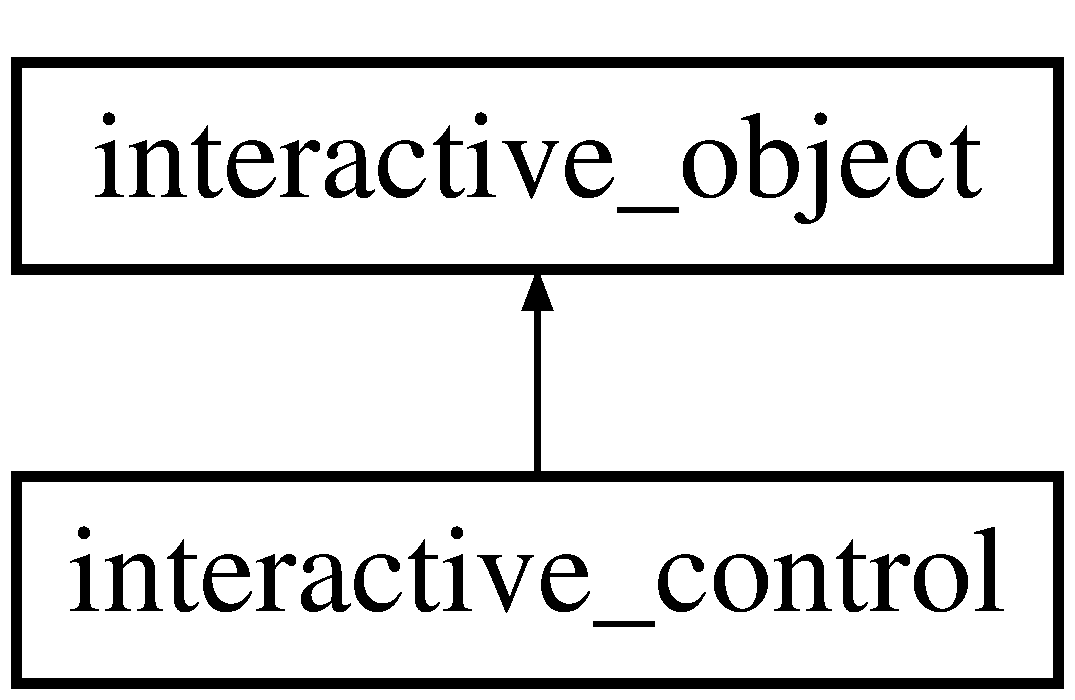
\includegraphics[height=2.000000cm]{structinteractive__control}
\end{center}
\end{figure}
\subsection*{Public Attributes}
\begin{DoxyCompactItemize}
\item 
\mbox{\Hypertarget{structinteractive__control_a60e147a9d4ae7f433a8b6f21daf3d5b4}\label{structinteractive__control_a60e147a9d4ae7f433a8b6f21daf3d5b4}} 
const char $\ast$ {\bfseries kind}
\item 
\mbox{\Hypertarget{structinteractive__control_a5b791bc356f723edcc3bd5c0e6a0365c}\label{structinteractive__control_a5b791bc356f723edcc3bd5c0e6a0365c}} 
size\+\_\+t {\bfseries kind\+Length}
\end{DoxyCompactItemize}


The documentation for this struct was generated from the following file\+:\begin{DoxyCompactItemize}
\item 
source/interactivity.\+h\end{DoxyCompactItemize}

\hypertarget{structinteractive__group}{}\section{interactive\+\_\+group Struct Reference}
\label{structinteractive__group}\index{interactive\+\_\+group@{interactive\+\_\+group}}
Inheritance diagram for interactive\+\_\+group\+:\begin{figure}[H]
\begin{center}
\leavevmode
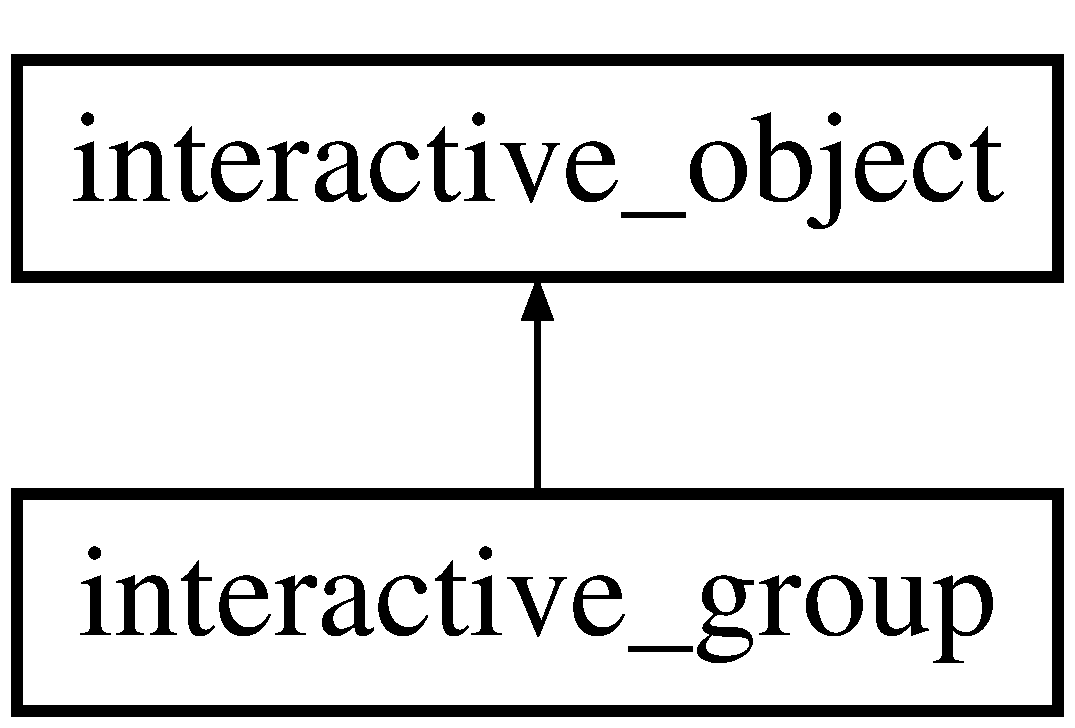
\includegraphics[height=2.000000cm]{structinteractive__group}
\end{center}
\end{figure}
\subsection*{Public Attributes}
\begin{DoxyCompactItemize}
\item 
\mbox{\Hypertarget{structinteractive__group_abc4b7f7f22871d5cc955fea0f0a13343}\label{structinteractive__group_abc4b7f7f22871d5cc955fea0f0a13343}} 
const char $\ast$ {\bfseries scene\+Id}
\item 
\mbox{\Hypertarget{structinteractive__group_a61c79cda8f163f6b0bb2e5147af15c56}\label{structinteractive__group_a61c79cda8f163f6b0bb2e5147af15c56}} 
size\+\_\+t {\bfseries scene\+Id\+Length}
\end{DoxyCompactItemize}


The documentation for this struct was generated from the following file\+:\begin{DoxyCompactItemize}
\item 
source/interactivity.\+h\end{DoxyCompactItemize}

\hypertarget{structinteractive__input}{}\section{interactive\+\_\+input Struct Reference}
\label{structinteractive__input}\index{interactive\+\_\+input@{interactive\+\_\+input}}
\subsection*{Classes}
\begin{DoxyCompactItemize}
\item 
struct \mbox{\hyperlink{structinteractive__input_1_1button_data}{button\+Data}}
\item 
struct \mbox{\hyperlink{structinteractive__input_1_1coordinate_data}{coordinate\+Data}}
\end{DoxyCompactItemize}
\subsection*{Public Attributes}
\begin{DoxyCompactItemize}
\item 
\mbox{\Hypertarget{structinteractive__input_ad6d5f6119bff198fffdbf80983ef1116}\label{structinteractive__input_ad6d5f6119bff198fffdbf80983ef1116}} 
\mbox{\hyperlink{structinteractive__control}{interactive\+\_\+control}} {\bfseries control}
\item 
\mbox{\Hypertarget{structinteractive__input_aeac5c04960be1d26422b88a89841ac57}\label{structinteractive__input_aeac5c04960be1d26422b88a89841ac57}} 
interactive\+\_\+input\+\_\+type {\bfseries type}
\item 
\mbox{\Hypertarget{structinteractive__input_ade05a03d25ad8463dbcfea2afff74f03}\label{structinteractive__input_ade05a03d25ad8463dbcfea2afff74f03}} 
const char $\ast$ {\bfseries participant\+Id}
\item 
\mbox{\Hypertarget{structinteractive__input_a86b0c8a7eb41c0c8c7459864ddd44347}\label{structinteractive__input_a86b0c8a7eb41c0c8c7459864ddd44347}} 
size\+\_\+t {\bfseries participant\+Id\+Length}
\item 
\mbox{\Hypertarget{structinteractive__input_a5110157c84774df95dc3bcea8ad03a8c}\label{structinteractive__input_a5110157c84774df95dc3bcea8ad03a8c}} 
const char $\ast$ {\bfseries json\+Data}
\item 
\mbox{\Hypertarget{structinteractive__input_a369891885d6c82df711ffdf00ed9721b}\label{structinteractive__input_a369891885d6c82df711ffdf00ed9721b}} 
size\+\_\+t {\bfseries json\+Data\+Length}
\item 
\mbox{\Hypertarget{structinteractive__input_a7e8bdd69904486dcd857da3e6160a405}\label{structinteractive__input_a7e8bdd69904486dcd857da3e6160a405}} 
const char $\ast$ {\bfseries transaction\+Id}
\item 
\mbox{\Hypertarget{structinteractive__input_aad326d8f738cdac83280741e9c0f794e}\label{structinteractive__input_aad326d8f738cdac83280741e9c0f794e}} 
size\+\_\+t {\bfseries transaction\+Id\+Length}
\item 
\mbox{\Hypertarget{structinteractive__input_ab3ec7b6c529fe57cd0ce8c530377b1ae}\label{structinteractive__input_ab3ec7b6c529fe57cd0ce8c530377b1ae}} 
struct \mbox{\hyperlink{structinteractive__input_1_1button_data}{interactive\+\_\+input\+::button\+Data}} {\bfseries button\+Data}
\item 
\mbox{\Hypertarget{structinteractive__input_ad8791985437c89e8f86812110c48b786}\label{structinteractive__input_ad8791985437c89e8f86812110c48b786}} 
struct \mbox{\hyperlink{structinteractive__input_1_1coordinate_data}{interactive\+\_\+input\+::coordinate\+Data}} {\bfseries coordinate\+Data}
\end{DoxyCompactItemize}


The documentation for this struct was generated from the following file\+:\begin{DoxyCompactItemize}
\item 
source/interactivity.\+h\end{DoxyCompactItemize}

\hypertarget{structinteractive__object}{}\section{interactive\+\_\+object Struct Reference}
\label{structinteractive__object}\index{interactive\+\_\+object@{interactive\+\_\+object}}
Inheritance diagram for interactive\+\_\+object\+:\begin{figure}[H]
\begin{center}
\leavevmode
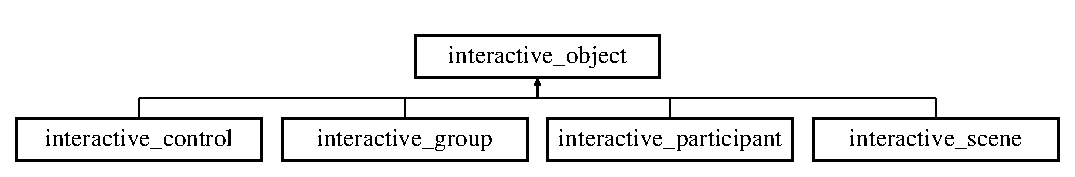
\includegraphics[height=1.931034cm]{structinteractive__object}
\end{center}
\end{figure}
\subsection*{Public Attributes}
\begin{DoxyCompactItemize}
\item 
\mbox{\Hypertarget{structinteractive__object_a4dc1bc79b2c49a36176df507feb750a7}\label{structinteractive__object_a4dc1bc79b2c49a36176df507feb750a7}} 
const char $\ast$ {\bfseries id}
\item 
\mbox{\Hypertarget{structinteractive__object_a787304bd5c30b4de4ff77f952c40f8c5}\label{structinteractive__object_a787304bd5c30b4de4ff77f952c40f8c5}} 
size\+\_\+t {\bfseries id\+Length}
\end{DoxyCompactItemize}


The documentation for this struct was generated from the following file\+:\begin{DoxyCompactItemize}
\item 
source/interactivity.\+h\end{DoxyCompactItemize}

\hypertarget{structinteractive__participant}{}\section{interactive\+\_\+participant Struct Reference}
\label{structinteractive__participant}\index{interactive\+\_\+participant@{interactive\+\_\+participant}}
Inheritance diagram for interactive\+\_\+participant\+:\begin{figure}[H]
\begin{center}
\leavevmode
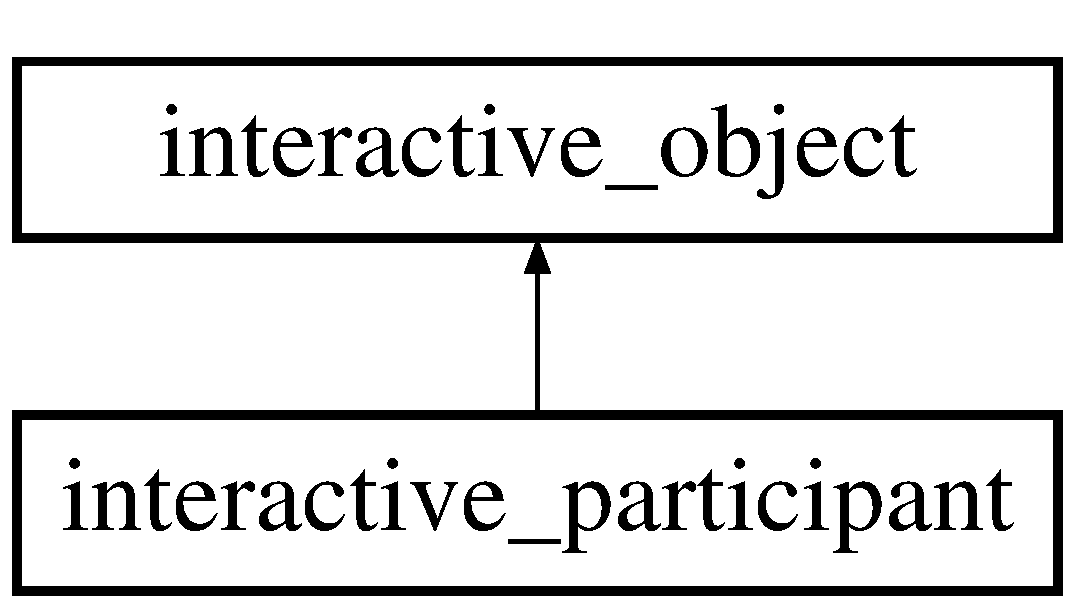
\includegraphics[height=2.000000cm]{structinteractive__participant}
\end{center}
\end{figure}
\subsection*{Public Attributes}
\begin{DoxyCompactItemize}
\item 
\mbox{\Hypertarget{structinteractive__participant_a9d27cfebd9602317dfaedadc9d302cd4}\label{structinteractive__participant_a9d27cfebd9602317dfaedadc9d302cd4}} 
unsigned int {\bfseries user\+Id}
\item 
\mbox{\Hypertarget{structinteractive__participant_ae78a284af5fe3abc48b858d432957857}\label{structinteractive__participant_ae78a284af5fe3abc48b858d432957857}} 
const char $\ast$ {\bfseries user\+Name}
\item 
\mbox{\Hypertarget{structinteractive__participant_ae31529a18da7df930653ce7be3a98472}\label{structinteractive__participant_ae31529a18da7df930653ce7be3a98472}} 
size\+\_\+t {\bfseries username\+Length}
\item 
\mbox{\Hypertarget{structinteractive__participant_a9463ba0a9e848db399d5b1b7258231c7}\label{structinteractive__participant_a9463ba0a9e848db399d5b1b7258231c7}} 
unsigned int {\bfseries level}
\item 
\mbox{\Hypertarget{structinteractive__participant_a7017d514fa39298a9404e7af0542eaa0}\label{structinteractive__participant_a7017d514fa39298a9404e7af0542eaa0}} 
unsigned long long {\bfseries last\+Input\+At\+Ms}
\item 
\mbox{\Hypertarget{structinteractive__participant_a1bbde35f772071a8887ccc6b66787194}\label{structinteractive__participant_a1bbde35f772071a8887ccc6b66787194}} 
unsigned long long {\bfseries connected\+At\+Ms}
\item 
\mbox{\Hypertarget{structinteractive__participant_aa1fa34e7b328bb17a0e89e6b9613be5a}\label{structinteractive__participant_aa1fa34e7b328bb17a0e89e6b9613be5a}} 
bool {\bfseries disabled}
\item 
\mbox{\Hypertarget{structinteractive__participant_af3b3c838023579396e4a96ce5e962c60}\label{structinteractive__participant_af3b3c838023579396e4a96ce5e962c60}} 
const char $\ast$ {\bfseries group\+Id}
\item 
\mbox{\Hypertarget{structinteractive__participant_a76fae5d8de8d655451658d9711227d98}\label{structinteractive__participant_a76fae5d8de8d655451658d9711227d98}} 
size\+\_\+t {\bfseries group\+Id\+Length}
\end{DoxyCompactItemize}


The documentation for this struct was generated from the following file\+:\begin{DoxyCompactItemize}
\item 
source/interactivity.\+h\end{DoxyCompactItemize}

\hypertarget{structinteractive__scene}{}\section{interactive\+\_\+scene Struct Reference}
\label{structinteractive__scene}\index{interactive\+\_\+scene@{interactive\+\_\+scene}}
Inheritance diagram for interactive\+\_\+scene\+:\begin{figure}[H]
\begin{center}
\leavevmode
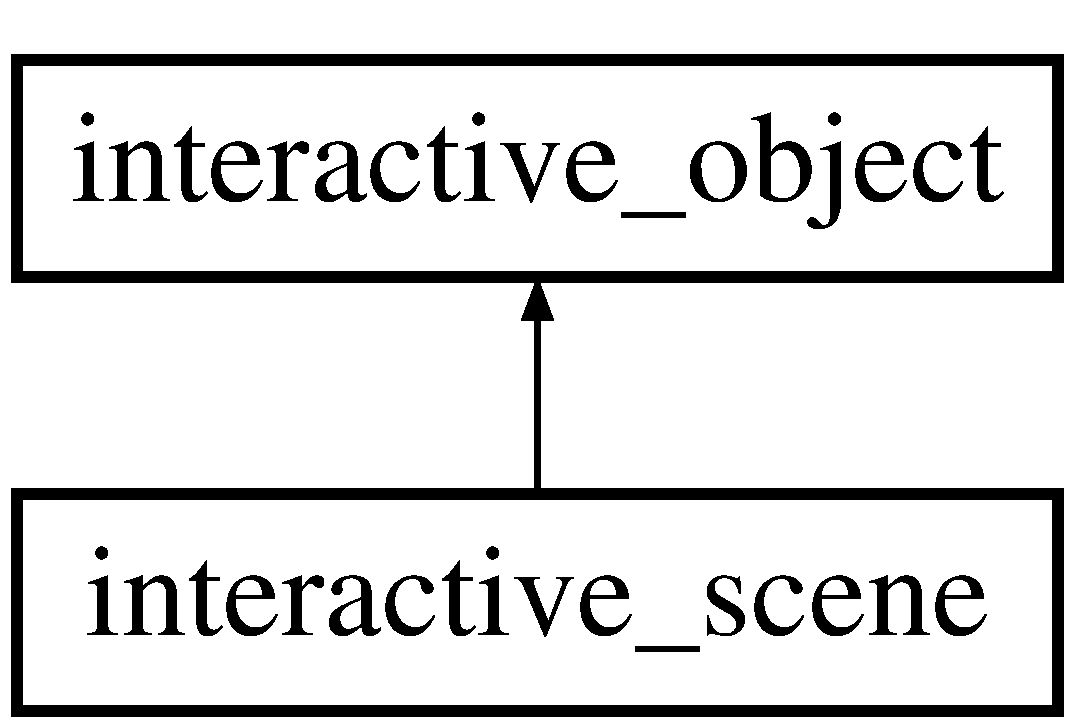
\includegraphics[height=2.000000cm]{structinteractive__scene}
\end{center}
\end{figure}
\subsection*{Additional Inherited Members}


The documentation for this struct was generated from the following file\+:\begin{DoxyCompactItemize}
\item 
source/interactivity.\+h\end{DoxyCompactItemize}

%--- End generated contents ---

% Index
\backmatter
\newpage
\phantomsection
\clearemptydoublepage
\addcontentsline{toc}{chapter}{Index}
\printindex

\end{document}
